% Copyright 2016 - 2023 Bas van Meerten and Wouter Franssen
%
%This file is part of ssNake.
%
%ssNake is free software: you can redistribute it and/or modify
%it under the terms of the GNU General Public License as published by
%the Free Software Foundation, either version 3 of the License, or
%(at your option) any later version.
%
%ssNake is distributed in the hope that it will be useful,
%but WITHOUT ANY WARRANTY; without even the implied warranty of
%MERCHANTABILITY or FITNESS FOR A PARTICULAR PURPOSE.  See the
%GNU General Public License for more details.
%
%You should have received a copy of the GNU General Public License
%along with ssNake. If not, see <http://www.gnu.org/licenses/>.

\documentclass[11pt,a4paper]{article}
% Copyright 2016 - 2020 Bas van Meerten and Wouter Franssen
%
%This file is part of ssNake.
%
%ssNake is free software: you can redistribute it and/or modify
%it under the terms of the GNU General Public License as published by
%the Free Software Foundation, either version 3 of the License, or
%(at your option) any later version.
%
%ssNake is distributed in the hope that it will be useful,
%but WITHOUT ANY WARRANTY; without even the implied warranty of
%MERCHANTABILITY or FITNESS FOR A PARTICULAR PURPOSE.  See the
%GNU General Public License for more details.
%
%You should have received a copy of the GNU General Public License
%along with ssNake. If not, see <http://www.gnu.org/licenses/>.


\usepackage[british]{babel}
\usepackage{graphicx,booktabs,listings,amsmath,ifthen,pgfplots,pgfplotstable}
\usepackage[small,bf,nooneline]{caption}
\usepackage{subcaption,longtable}
\usepackage[sort&compress,numbers]{natbib}
\usepackage{tikz,tikz-3dplot}
\usetikzlibrary{backgrounds,arrows,calc}
\usepackage{mathtools}
\usepackage[nottoc]{tocbibind}%adds bibliography to table of contents.
\graphicspath{{./images/}}
%\setlength{\textwidth}{453pt} %597 pt is the a4 paperwidth. Minus 2 in margin. 72 pt = 1 in
%\setlength{\hoffset}{-\oddsidemargin}
%\setlength{\voffset}{-30pt} %
%\setlength{\textheight}{651 pt} %a4 height 845 pt minus 2* total headheight. In this case 2*88pt
%% examine margines via the layout package. Use command \layout{} in document to draw a picture.
%\setlength{\parindent}{0.5 cm}
%\setlength{\parskip}{0 cm}
%\usepackage[left=82pt,right=62pt,top=95pt,bottom=95pt,footnotesep=0.5cm]{geometry}
%\setlength{\headheight}{14pt}

%define colours--------------------
%dark
\usepackage{xcolor}
\definecolor{MyGrayD}{RGB}{1,1,1}
\definecolor{MyRedD}{RGB}{237,45,46}
\definecolor{MyGreenD}{RGB}{0,140,71}
\definecolor{MyBlueD}{RGB}{24,89,169}
\definecolor{MyOrangeD}{RGB}{243,125,34}
\definecolor{MyPurpleD}{RGB}{102,44,145}
\definecolor{MyBrownD}{RGB}{161,29,32}
\definecolor{MyPinkD}{RGB}{179,56,147}
%normal
\definecolor{MyGray}{RGB}{114,114,114}
\definecolor{MyRed}{RGB}{241,89,95}
\definecolor{MyGreen}{RGB}{121,195,106}
\definecolor{MyBlue}{RGB}{89,154,211}
\definecolor{MyOrange}{RGB}{249,166,90}
\definecolor{MyPurple}{RGB}{158,102,171}
\definecolor{MyBrown}{RGB}{205,112,88}
\definecolor{MyPink}{RGB}{215,127,179}
%light
\definecolor{MyGrayL}{RGB}{204,204,204}
\definecolor{MyRedL}{RGB}{242,174,172}
\definecolor{MyGreenL}{RGB}{216,228,170}
\definecolor{MyBlueL}{RGB}{184,210,235}
\definecolor{MyOrangeL}{RGB}{242,209,176}
\definecolor{MyPurpleL}{RGB}{212,178,211}
\definecolor{MyBrownL}{RGB}{221,184,169}
\definecolor{MyPinkL}{RGB}{235,191,217}
%----------------------------------

%Figure ref with hyperref
\newcommand{\fref}[1]{\hyperref[#1]{Figure \ref*{#1}}}
\newcommand{\sref}[1]{\hyperref[#1]{Section \ref*{#1}}}
\newcommand{\tref}[1]{\hyperref[#1]{Table \ref*{#1}}}

%Makes a new command for figures with input values: filename, width(times linewidth),
% caption and label.
\newcommand{\onefigure}[4]{
\setlength{\captionwidth}{#2\linewidth}
\begin{figure}
\includegraphics[width=#2\linewidth]{#1}
\centering
\parbox{\linewidth}{\caption{#3}
\label{#4}}
\end{figure}
}

%Makes a new command for tikz figures with input values: tikz commands, 
% caption and label.
\newcommand{\onetikz}[3]{
\settowidth{\captionwidth}{#1}
\ifthenelse{\lengthtest{\captionwidth<0.7\linewidth}}{\setlength{\captionwidth}{0.7\linewidth}}{}

\begin{figure}
\centering
#1
\centering
\parbox{\linewidth}{\caption{#2}
\label{#3}}
\end{figure}
}

%Makes a new command for two figures next to each other with input values: filename1, caption1, label1,filename2, caption2 and label2. Figure width is set to 0.47\linewidth and the space between the figures is filled with \hfill so the sides of the figures align with to edge of the line.
\newcommand{\twofigure}[6]{
\setlength{\captionwidth}{\linewidth}
\begin{figure*}[ht!]
\begin{minipage}[t]{0.47\linewidth}
\includegraphics[width=\linewidth]{#1}
\centering
\caption{#2}
\label{#3}
\end{minipage}
\hfill
\begin{minipage}[t]{0.47\linewidth}
\centering
\includegraphics[width= \linewidth]{#4}
\centering
\caption{#5}
\label{#6}
\end{minipage}
\end{figure*}
}


%Makes a new command for a table with caption witdh equal to the total table width. Input: tabular, caption and label. Example:
%\onetable{
%\begin{tabular}{ccc}
%a&b&c\\
%\hline
%1&1&1\\
%1&1&1\\
%1&1&1\\
%\end{tabular}
%{The caption.}
%{tab:table1}
%}
\newcommand{\onetable}[3]{
\settowidth{\captionwidth}{#1}
\ifthenelse{\lengthtest{\captionwidth<0.7\linewidth}}{\setlength{\captionwidth}{0.7\linewidth}}{}
\begin{table}
\caption{#2}
\vspace{-0.24cm} %Puts caption close to toprule
\label{#3}
\centering
#1
\end{table}
}

%Makes a long table with captionwidth equal to tablewidth. It takes the following arguments:
%1: Column specifier (e.g. cccc)
%2: Caption
%3: Label
%4: First head (i.e. first row of regular table)
%5: Head of consecutive pages
%6: Foot of pagebreak
%7: Lastfoot (e.g. \midrule)
%8: Body of table
\newcommand{\onelongtable}[8]{
\begin{center}
\settowidth{\captionwidth}{
\begin{tabular}{#1}
#4
#8
\end{tabular}} % This ends the captionwidth part. Next comes the real table.

\begin{longtable}{#1}
\caption{#2}\\
\vspace{-0.74cm} %Puts caption close to toprule
\label{#3}\\

#4
\endfirsthead

#5
\endhead

#6
\endfoot

#7
\endlastfoot

#8
\end{longtable}
\end{center}}




%1:pgfplots code
%2:width
%3:caption
%4:label
\newcommand{\pgfplotsfigure}[4]{
\pgfplotsset{width=#2\linewidth}
\setlength{\captionwidth}{#2\linewidth}
\begin{figure}[t]
\centering
#1
\centering
\parbox{\linewidth}{\caption{#3}
\label{#4}}
\end{figure}
}


\usepackage[bitstream-charter]{mathdesign}
\usepackage[T1]{fontenc}
\usepackage[protrusion=true,expansion,tracking=true]{microtype}
\pgfplotsset{compat=1.7,/pgf/number format/1000 sep={}, axis lines*=left,axis line style={gray},every outer x axis line/.append style={-stealth'},every outer y axis line/.append style={-stealth'},tick label style={font=\small},label style={font=\small},legend style={font=\footnotesize}}
\usepackage{colortbl}
\usepackage{listings}


%Set section font
\usepackage{sectsty}
\allsectionsfont{\color{black!70}\fontfamily{SourceSansPro-LF}\selectfont}
%--------------------


%Set toc fonts
\usepackage{tocloft}
%\renewcommand\cftchapfont{\fontfamily{SourceSansPro-LF}\bfseries}
\renewcommand\cfttoctitlefont{\color{black!70}\Huge\fontfamily{SourceSansPro-LF}\bfseries}
\renewcommand\cftsecfont{\fontfamily{SourceSansPro-LF}\selectfont}
%\renewcommand\cftchappagefont{\fontfamily{SourceSansPro-LF}\bfseries}
\renewcommand\cftsecpagefont{\fontfamily{SourceSansPro-LF}\selectfont}
\renewcommand\cftsubsecfont{\fontfamily{SourceSansPro-LF}\selectfont}
\renewcommand\cftsubsecpagefont{\fontfamily{SourceSansPro-LF}\selectfont}
%--------------------

%Define header/foot
\usepackage{fancyhdr}
\pagestyle{fancy}
\fancyhead[LE,RO]{\fontfamily{SourceSansPro-LF}\selectfont \thepage}
\fancyhead[LO,RE]{\fontfamily{SourceSansPro-LF}\selectfont \leftmark}
\fancyfoot[C]{}
%--------------------

%remove page number from first chapter page
\makeatletter
\let\ps@plain\ps@empty
\makeatother
%----------------------
\usepackage{blindtext, color}
\definecolor{gray75}{gray}{0.75}
\newcommand{\hsp}{\hspace{20pt}}



\usepackage[hidelinks,colorlinks,allcolors=blue, pdftitle={The ssNake reference manual},pdfauthor={W.M.J.\ Franssen}]{hyperref}

\interfootnotelinepenalty=10000 %prevents splitting of footnote over multiple pages
\linespread{1.2}

%\usepgfplotslibrary{external}%creates all external tikz images that are included.
%\tikzexternalize[shell escape=-enable-write18]%activate externalization
%\tikzsetexternalprefix{GeneratedFigures/}
%\tikzset{external/force remake} %Enable forced remake



\begin{document}
%\newgeometry{left=72pt,right=72pt,top=95pt,bottom=95pt,footnotesep=0.5cm}
% Copyright 2016 - 2019 Bas van Meerten and Wouter Franssen
%
%This file is part of ssNake.
%
%ssNake is free software: you can redistribute it and/or modify
%it under the terms of the GNU General Public License as published by
%the Free Software Foundation, either version 3 of the License, or
%(at your option) any later version.
%
%ssNake is distributed in the hope that it will be useful,
%but WITHOUT ANY WARRANTY; without even the implied warranty of
%MERCHANTABILITY or FITNESS FOR A PARTICULAR PURPOSE.  See the
%GNU General Public License for more details.
%
%You should have received a copy of the GNU General Public License
%along with ssNake. If not, see <http://www.gnu.org/licenses/>.

\begin{titlepage}
\begin{center}




% Upper part of the page
{\Huge The ssNake reference manual}
\vfill
\large Wouter Franssen \& Bas van Meerten

\vspace{1cm}
\large Version 1.2b
\vfill

\includegraphics[width=0.5\textwidth]{Images/logo.pdf}\

\vfill
\vfill
% Bottom of the page
{\large \today}

\end{center}

\end{titlepage}


\thispagestyle{empty}
\newpage
\mbox{}

%\restoregeometry

\pagenumbering{roman}
%\pagestyle{empty}
\renewcommand\cfttoctitlefont{\color{black}\Huge\fontfamily{SourceSansPro-LF}\bfseries}
\microtypesetup{protrusion=false} % disables protrusion locally in the document
\setcounter{tocdepth}{2}
\tableofcontents % prints Table of Contents
\microtypesetup{protrusion=true} % enables protrusion
\addtocontents{toc}{\protect\thispagestyle{empty}}
%\pagestyle{plain}

\renewcommand\cfttoctitlefont{\color{black!70}\Huge\fontfamily{SourceSansPro-LF}\bfseries}


\pagenumbering{arabic}
\section{Introduction}
ssNake (solid state NMR analysation and knowledge engine) is a versatile program for the processing
and analysis of NMR data. It is aimed at solid state NMR. ssNake is written in the Python programming
language, and is cross-platform and open-source (GPL3 licence). ssNake focusses at manual interactive
processing of data (compared to other software which tries to automate as much as possible).

\subsection{Documentation structure}
Most of this documentation discusses the menu items as can be found in ssNake. Sometimes, extra
Sections are inserted to explain underlying mechanisms of ssNake. For a general impression on how to
work with ssNake, the tutorial that is bundled with ssNake is a better place to start. Detailed
explanation of all the options can then be found in this Reference Manual. More advanced tutorials
can be found online, on the dedicated github page:
\url{https://github.com/smeerten/ssnake_tutorials}.


\section{Running ssNake}
\subsection{Python and library versions}
ssNake has been programmed to run on both the python 2.x and 3.x. ssNake should run on python
versions starting from 2.7 and 3.4.
For the library version, the following are needed:
\begin{itemize}
  \item  \texttt{numpy} $>=$ 1.11.0
  \item  \texttt{matplotlib} $>=$ 1.5.0
  \item  \texttt{scipy} $>=$ 0.14.1
\end{itemize}
ssNake also needs the \texttt{PyQt} (version 4 or 5) and \texttt{h5py} libraries.

\subsection{Installing}
\subsubsection{Linux}
On Linux, ssNake can be most efficiently run using the python libraries that are in the
repositories. For Ubuntu, these can be installed by running:
\begin{verbatim}
sudo apt install python python-numpy python-matplotlib python-scipy
python-pyqt5 python-h5py
\end{verbatim}
Navigating to the \texttt{ssNake/src} directory in a terminal, ssNake can then be run
by executing \texttt{python ssNake.py}.

\subsubsection{Windows}
On Windows, the relevant python libraries can be installed by installing \texttt{anaconda}:
\url{https://www.anaconda.com/download/}. If you do not have another python version installed
already, make sure to add anaconda to the \texttt{path} during the install. In this case, ssNake can
be run by executing the \texttt{WindowsRun.bat} file in the \texttt{ssNake/src} directory. Destktop
and start menu shortcuts to this file can be created by executing the \texttt{WindowsInstall.vbs}
file.

If you already have other version of python installed, adding anaconda to the \texttt{path} might
create issues. Do not do this in this case. When not added to the path, the \texttt{WindowsRun.bat}
should be edited in such a way that \texttt{pythonw} is replaced with the path to your
\texttt{pythonw.exe} executable in the anaconda install directory. Note that, when updating ssNake,
this file will be replaced.

\subsubsection{OS X}
On OS X, the relevant python libraries can be installed by installing \texttt{anaconda}:
\url{https://www.anaconda.com/download/}. Navigating to the \texttt{ssNake/src} directory in a terminal, ssNake can then be run
by \texttt{anacondapython ssNake.py}, with \texttt{anacondapython} replaced by the path to your
anaconda python executable.



\section{Main window}
\autoref{fig:interface} shows the main interface of ssNake. Below, each element will be described.

\begin{figure}[t]
  \centering
  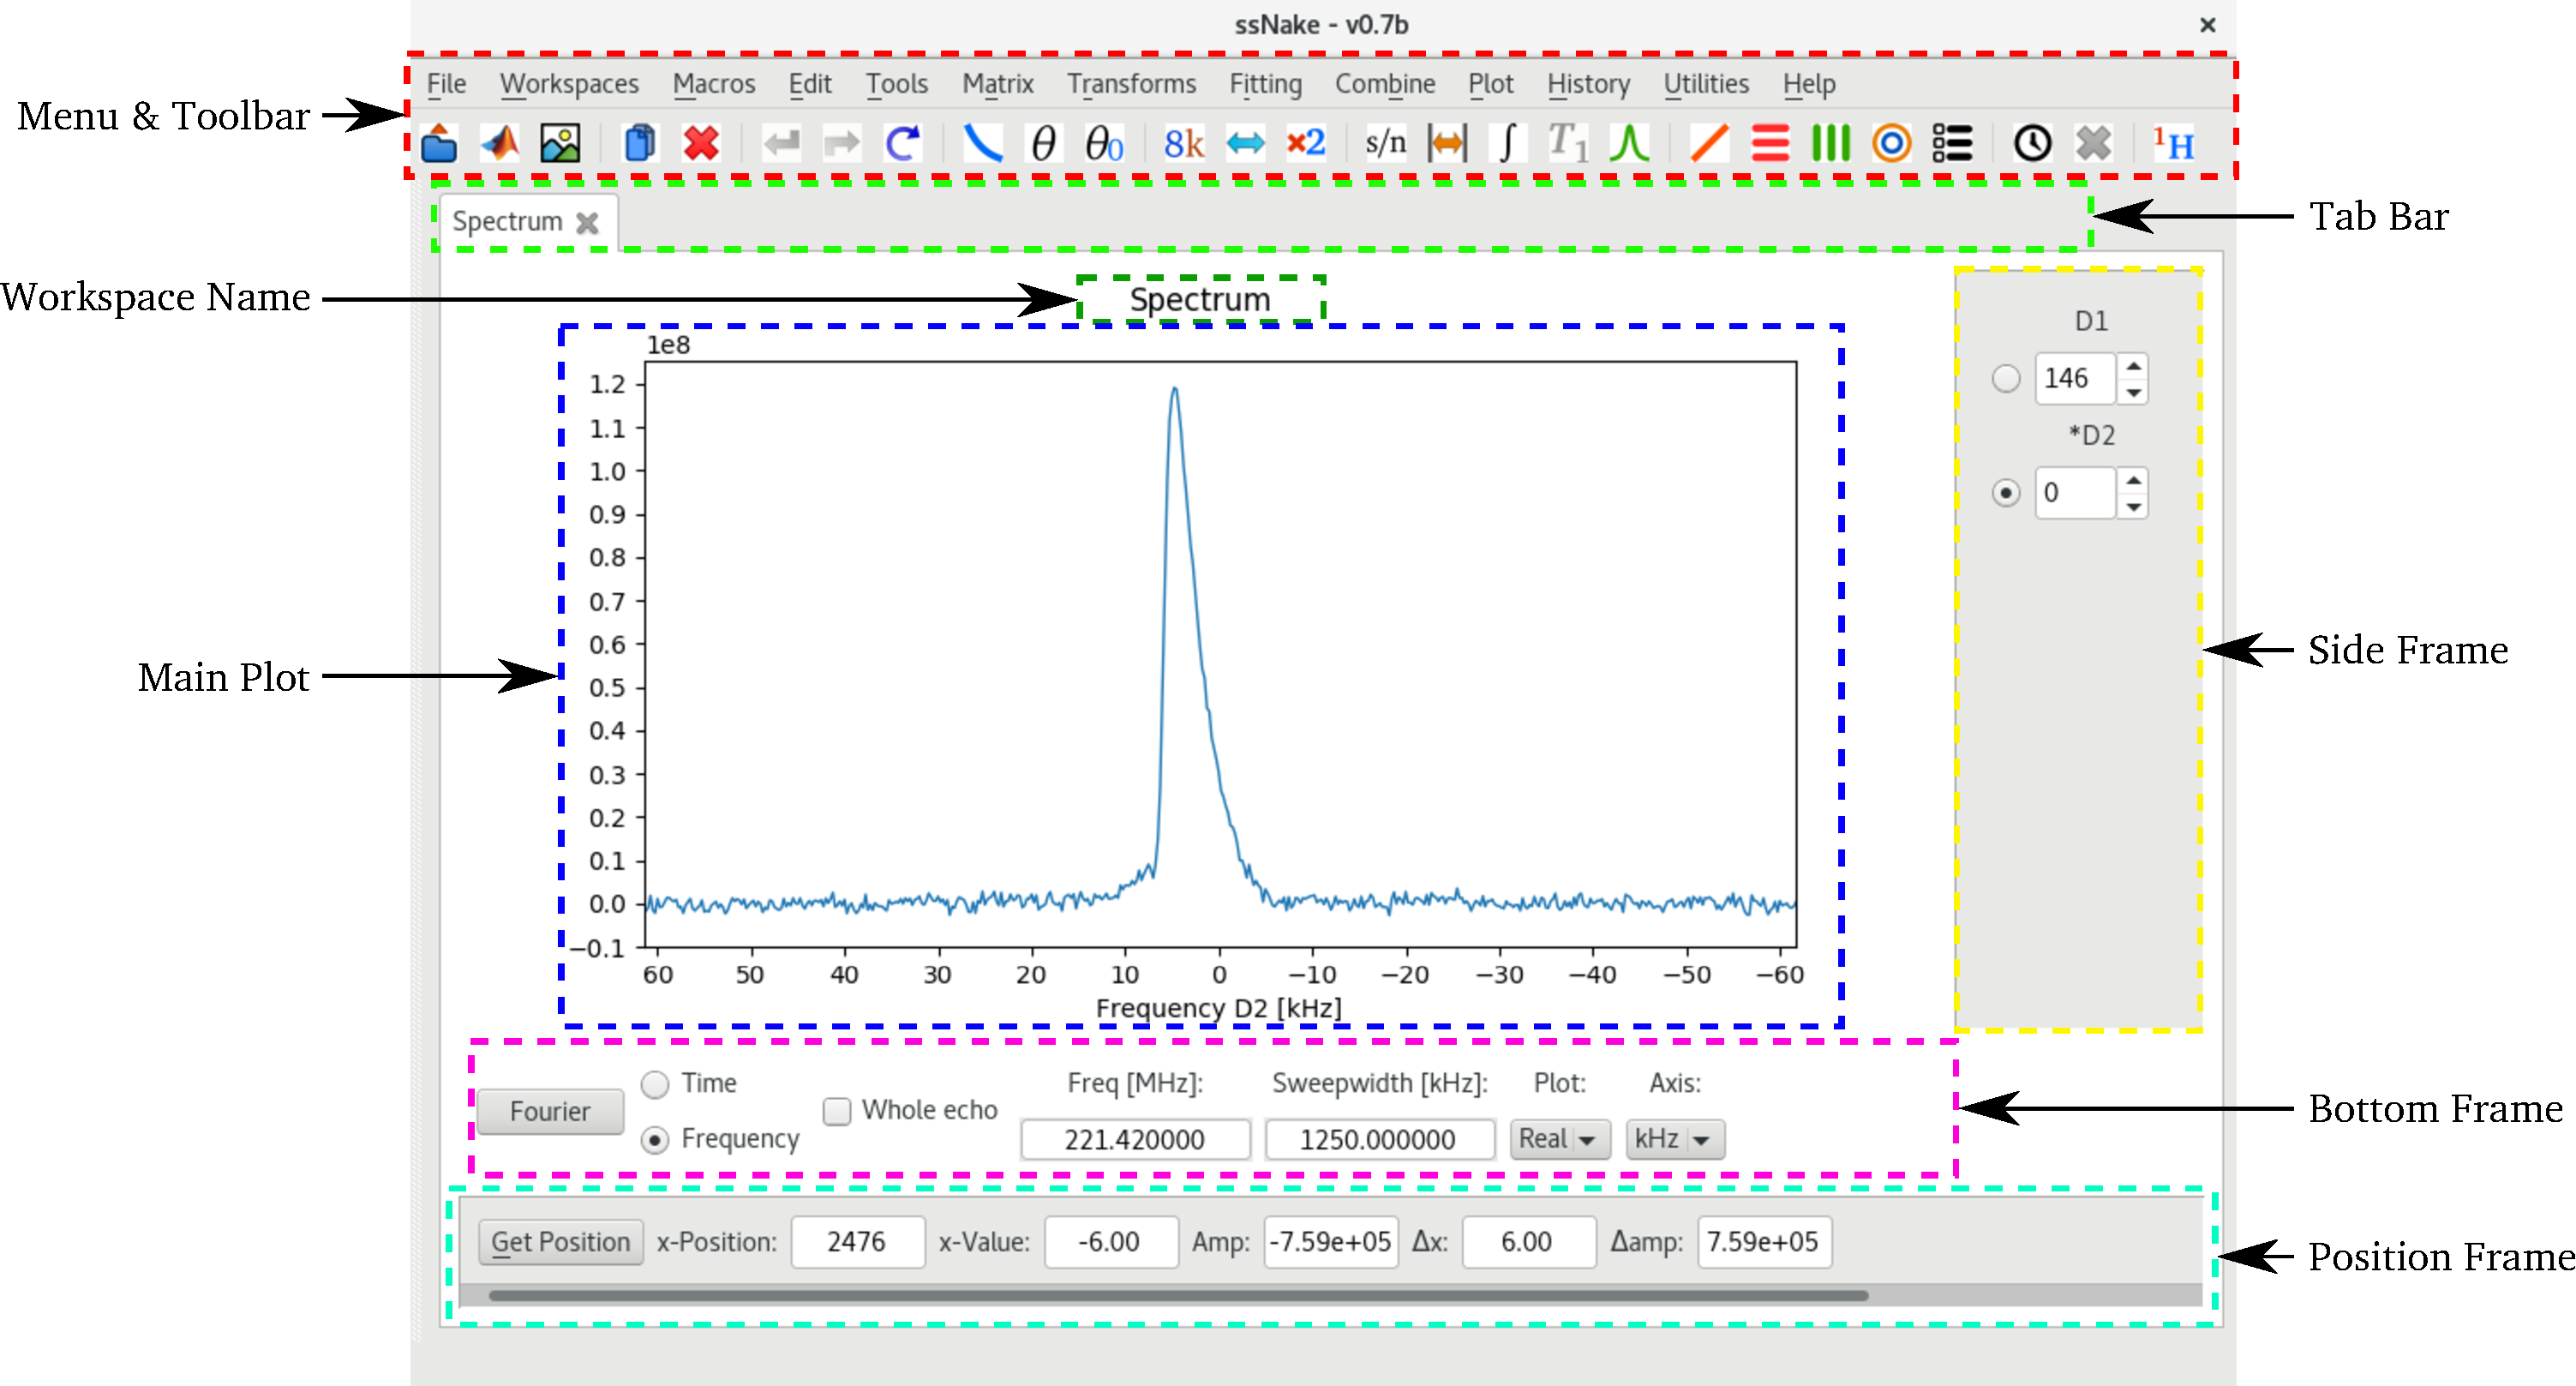
\includegraphics[width=\linewidth]{Images/Interface.pdf}
  \caption{Main interface of ssNake.}
  \label{fig:interface}
\end{figure}

\subsection{Menu \& Toolbar}
This area show  the menu and the toolbar. The toolbar holds a number of the actions that can be
found in the Menu. The actions in the toolbar can be changed via the \texttt{Preferences}.




\subsection{Tab Bar}
Each data set that is opened in ssNake opens in its own tab (i.e. Workspace). Switching the active
workspace can be done by clicking on the relevant tab, or by using keyboard shortcuts (found in the
Workspaces menu). Closing workspaces can be done by clicking on the cross of the tab, or by clicking
the middle mouse button when the mouse pointer is hovering over the tab name.

\subsection{Main Plot}
In the centre of the interface is the Main Plot. This shows the spectrum or FID of the current
workspace (i.e. tab). The view of this plot can be changed by using the mouse controls described
below. Some of the processing tools described later on rely on user input given by clicking in the
Main Plot (i.e. selecting a region).

\subsubsection{Mouse controls}
There are several ways to control the display of the current spectrum or FID in the main window
using the mouse. Below, a list of these is given:

\begin{itemize}
\item Dragging a box while holding the left mouse button creates a zoombox, and will zoom to that region.
\item Dragging while holding the right mouse button drags (i.e.\ pans) the spectrum. Doing this while holding the Control button pans only the x-axis, holding Shift pans only the y-axis.
\item Double clicking with the right mouse button resets the view to fit the whole plot (both x and y).
\item Scrolling with the mouse wheel zooms the y-axis. Doing this while also holding the right mouse button zooms the x-axis. By holding Control the zooming will use a larger step size. In a Contour plot, the projections can also be zoomed by scrolling when the mouse pointer is over one of these plots. The top projection can be zoomed using normal scrolling, while the right projection can be zoomed using scrolling while holding the right mouse button.
\item \textit{Special}: Scrolling while holding shift changes the spacing between the different plots in the Array or Stack plot. In the Contour plot, the contour levels are zoomed.
\end{itemize}

Having an input window open (e.g. the phasing window, see below) does not prevent the use of these zoom controls. However, some tools require left clicking in the spectrum to select data points. In these cases, the zoom-box (dragging while holding the left mouse button) is disabled.

\subsection{Bottom Frame}
The bottom frame is the frame below the current data display. It consist of two parts: one with data parameters (and started by the `Fourier' button), and the `Get Position' frame. The features of these frames are explained below.

\subsubsection*{Data parameters}
The data parameter frame features the following elements:
\begin{itemize}
\item The Fourier button: performs a forward or inverse fft depending on Time/Frequency toggle. If the current setting is Time, it does a forward transform (and fft shift), if it is Frequency it does an inverse transform.
\item Time/Frequency toggle: displays whether the current data is an FID (Time) or Spectrum (Frequency). It is usually not necessary to manually change this, as this is done automatically.
\item Whole echo: specifies if a whole echo transform should be done. This is set by using the swap echo tool from the Tools menu (see below). When enabled, several tools respond differently (e.g. Apodizing and Set Size).
\item Freq [MHz]: The centre frequency of the current spectrum dimension in MHz. Note that this value can be different from the Reference frequency, which specifies the zero frequency of the spectrum.
\item Sweepwidth [kHz]: The spectral width of the current spectrum dimension in kHz.
\item Plot: A dropdown menu specifying how the data should be plot. It has four options: Real, Imag, Both and Abs. Real: plots only the real part of the complex data. Imag: plots only the imaginary part. Both: plots both the real and imaginary part of the data in different colours. Abs: plots the absolute value of the data. Note that this only toggles the \textit{view} of the current data. Changing the data itself can be done via the Tools menu.
\item Axis: Dropdown menu to change the units of the current x-axis. For a time axis, s, ms and $\muup$ are supported. For the frequency axis: Hz, kHz, MHz and ppm.
\item \textit{Special}: Axis2: changes the unit of the y-axis in a 2D contour plot.
\end{itemize}

\subsubsection*{Position Frame}
The Position frame is the frame in which the properties of a specific data point can be viewed.
Pushing the `Get Position'  button and then left clicking on a specific point in the spectrum or FID
prints this data. The `Get Position frame' then displays the number of the data point you clicked on
(note that in a spectrum the data goes from right to left!), the x and amplitude (y) value of this
data point and the difference with your last pick. In a Contour plot, the amplitude actually codes
for the z value, and there now is a separate y value box (and corresponding y difference) as well as
the index of the point along the y dimension. In most plot types, a dashed vertical line is shown at
the position of the cursor to aid in the selection of a point. In the Contour plot, a horizontal
line is also shown.

\subsection{Side Frame}
On the right side of the spectrum, there is an additional frame in some cases called the Side Frame. In this, special settings for the current plot type can be set, as well as the dimension along which the data should be plot. For a regular 1D spectrum of 1D data there are no additional options, and the Side Frame is not shown. The description of the elements that are shown in the Side Frame are explained in the section on the different plot types. However, the common feature for multidimensional data (i.e. the dimension selector) shall be explained here.

\subsubsection*{The dimension selector}
For data that has more than 1 dimension, a dimension selector is shown in the Side Frame. For each dimension (labelled D1 to D$n$, with $n$ the number of dimensions) there is a radio button and an input box. The radio button indicates which dimension is plot in the main window. For 2D plots or arrayed plots, both the direct and the indirect dimension have to be selected. For all the dimensions of which the radio button is not selected, the input box is used to define which trace is plot. Take for example a series of ten 1D spectra with 1024 points per spectrum. The total data size is now 10x1024 (D1xD2). Note that the direct spectral dimension is always the last dimension. In a regular view of the first spectrum of this series, the radio button below D2 should be selected (as is the default setting). The number in the box next to D1 then determines which of the 10 spectra to plot. If this value is 0, the first spectrum is plot (note that ssNake uses the Python rules for array indexing, and that 0 is the first index). As we have ten spectra, 9 is the last. Similar to Python indexing, negative values can be used for reverse indexing (-1 is the last, -2 is the second to last, etc.). Using the up and down buttons next to the input box below D1, the spectra can be cycled. Also, scrolling with the scroll wheel when the mouse is on top of the box can be used.

For data with more dimensions, the idea is essentially the same. Note that ssNake always applies processing commands on the active (selected) dimension. If two dimensions need to be selected (as in an array or contour plot), the leftmost radio button is the selected dimension for operations.

\subsection{Message bar}
The bottommost part of the ssNake window is the message bar. Any error messages will be printed here
in red. Warnings about wrong inputs will be displayed in black. For both type of messages the same
applies: they are shown for several seconds, and then disappear. If some tool is not responding, it
is therefore wise to check the message bar for messages.


\subsection{File Tree}
On the left side of the Main Window, there is a file tree, which can be used to browse the computer,
and open data. Data can be loaded by right clicking on a file or folder, and selecting `Load
Directory' or `Load File'. Alternatively, clicking on the folder or file name using the middle mouse
button opens it directly.

The File Tree can be closed bu double clicking on the separator between the Tree and the Main Plot,
or by clicking with the middle mouse button.







\section{Pop-up windows}
Many of the operations that can be performed in ssNake give a pop-up window in which the user can
supply additional information. An example of this is the phasing window, in which the user can
supply values for the first and second order phasing that should be applied to the NMR data. When
such a pop-up window is active most of the Main Window is locked. When closing the pop-up window,
the interface is enabled again. This makes sure that there is no interference between the different
actions.

Most pop-up windows have an `Ok' and a `Cancel' button. Pushing `Ok' applies the operation to the
data set. Pushing `Cancel' returns to the Main Window without any alteration of the data. Is some
cases, the effect of the current operation can be previewed in the plot. This allows the user to
judge whether the operation (e.g. an amount of phasing) leads to the desired result. Choosing
`Cancel' returns to the original data. During the previewing, the mouse button zoom controls can
still be used. However, in cases where the left mouse button is used to select a position in the
plot, the `zoom box' option is not available during the preview. Previewing is usually quite fast,
as only the currently viewed part of the data is temporarily changed. On pushing `Ok' the operation
is applied to the full data set (if required).

\subsection{Single slice}
Some of the pop-up windows have a tickbox at the bottom that states `Single slice'. When this is
activated, the current operation only gets performed on the part of the data that is currently
viewed. Phasing a single spectrum in a 2D data set can for example be performed in this way.

\subsection{Keyboard modifiers}
Some of the pop-up windows have left `<' and right `>' arrow buttons. These can be used to lower or
raise the current value in an easy way. The step size of the buttons can be changed by holding
specific keys when left clicking on the button: `ctrl' gives x10 stepsize, `shift' gives x100, and
`ctrl + shift' gives x1000.


\section{File}
Using the ssNake load tools is quite easy. Go to File $\rightarrow$ Open. Navigating and double clicking on the desired file then loads the data. Many formats supported by ssNake (like Bruker and Varian) have their data in a folder, in which several files with a fixed name are present. For these formats, loading any of the files in this directory is accepted (ssNake searches for the expected files in the selected directory). Loading large data files might take some time, depending on your computer hardware.

When loading the data, the user is prompted to give in a name by which the workspace is identified (see the Workspaces section for more on this). The default name is the name of the file (or folder for data in which the filename is fixed). If the name already exists as a workspace, the name spectrum\textit{n} is used (with \textit{n} the lowest integer that is not in use).


\subsection{Formats}
ssNake is able to extract NMR data from a number of formats from several vendors. The following table summarizes the support.

\begin{center}
\begin{tabular}{lc}
\toprule
Name & Specification \\
\midrule
\rowcolor{gray!30!white}
Varian/Agilent & VnmrJ 2 and newer. \texttt{fid} and \texttt{data} (spectrum)\\
Bruker & Topspin and XWinNMR (\texttt{fid} \& \texttt{ser},\texttt{1r/i} \& \texttt{2rr/ii}) \\
\rowcolor{gray!30!white}
Bruker ParaVision & processed data (\texttt{2dseq})\\
Bruker minispec  & \texttt{.sig} file\\
\rowcolor{gray!30!white}
Bruker EPR & \texttt{.spc} and \texttt{.par} files. 1D and 2D.\\
JEOL Delta & 1D and 2D only at the moment \\
\rowcolor{gray!30!white}
Chemagnetics & -- \\
Magritek & Both 1D and 2D data \\
\rowcolor{gray!30!white}
SIMPSON & 1D and 2D, -ascii and -binary \\
JCAMP & 1D JCAMP-DX file\\
\rowcolor{gray!30!white}
DMFIT & \texttt{.txt}; 1D spectra only at the moment\\
Siemens ima & single voxel only\\
\rowcolor{gray!30!white}
JSON & ssNake JSON file (ascii)\\
Matlab & ssNake \texttt{.mat} file (binary)\\
\bottomrule
\end{tabular}
\end{center}

Generally, ssNake loads the raw data and searches for some variables (e.g. spectral width and spectrometer frequency). The above data formats do not support data with more then two dimensions in a nice way. Getting the higher dimensions is therefore not straightforward. ssNake treats this data as 2D, after which you can split the data yourselves using Matrix $\rightarrow$ Split.

\subsubsection*{Varian/Agilent}
Loading a Varian/Agilent fid file requires a \textit{procpar} file and a \textit{fid} file. From the \textit{procpar}, the spectral frequency and the spectral width in one or two dimensions is extracted. The \textit{fid} file is then checked for the version (VnmrJ 2 or 3) and the data is extracted from this file.

For processed data (\textit{data}, in the datdir folder for example) it searches for a \textit{procpar} file in that directory or in the parent folder, from which additional parameters are extracted.

\subsubsection*{Bruker}
The Bruker load first checks for the \textit{acqus} and \textit{acqu2s} files and extracts the number of points in both dimensions, the spectral widths and the spectral frequency. Also, the bitorder is checked, which describes the way the data is saved in the \textit{fid} or \textit{ser} file. Using this, the data is extracted.

Bruker processed spectra can be loaded from \textit{1r} and \textit{1i} files for 1D data, \textit{2rr} and \textit{2ii} for 2D data, and \textit{2rr} and \textit{2ir} for hypercomplex data. It additionally takes parameters from \textit{procs} or \textit{proc2s} files in that directory. Moreover, the spectral frequency is extracted from the \textit{acqus} and/or \textit{acqu2s} files located \textit{two directories up}.

\subsubsection*{Bruker ParaVision}
Loads processed data acquired via Bruker ParaVision. This feature is experimental at the moment. It need several files: \texttt{2dseq}, \texttt{d3proc} and \texttt{procs}.

\subsubsection*{Bruker minispec}
In some cases, the Bruker minispec also outputs a \texttt{.sig} data file. These can be loaded in ssNake, although this is experimental at the moment.

\subsubsection*{Bruker EPR}
Loads Bruker EPR data. Can load both 1D and and 2D (series of 1D data). Needs \texttt{.spc} and \texttt{.par} files.

\subsubsection*{JEOL Delta}
JEOL Delta data is contained in a single \texttt{.jdf} file. Currently only 1D and 2D data is
 supported. This is because we have no access to a JEOL spectrometer for testing
purposes. Please send us test files is you have any.

\subsubsection*{Chemagnetics}
Loading Chemagnetics data requires a \textit{acq} (and \textit{acq\_2} for 2D) and \textit{data} file. From the former, the number of points in both dimensions is extracted, the spectral widths and the spectral frequency. All the data points are then extracted form the \textit{data} file, and reshaped to a 2D array when necessary.

\subsubsection*{Magritek}
Magritek requires either two or three files: \textit{acqu.par} for the spectral variables, and a file that ends with \textit{.1d}. For 2D data, a file that ends in \textit{.2d} is also needed. As with the other formats, the number of data points in the two dimensions is extracted from the parameter file (along with the spectral data) and the binary data in the \textit{.1d} or \textit{.2d} is unpacked.

\subsubsection*{SIMPSON}
SIMPSON data files are plain text files, \textit{.fid} or \textit{.spe} as file extension. From the file, the number of points in both dimensions is extracted, and the spectral widths. The spectral frequency is \textit{not} included in the SIMPSON format, and is put at 0. SIMPSON files cannot contain a mixture of time and frequency data (both dimensions must be the same type). SIMPSON binary data is also supported, but not raw binary.

\subsubsection*{JCAMP}
JCAMP (or JCAMP-DX) is a general format for storing spectroscopic data. Although it can be applied to NMR data, it is inconvenient, especially for 2D data. ssNake therefore only supports 1D fid and spectrum data at the moment. As the JCAMP format support a wide variety of data formats, it depends on the specific file if it can be loaded into ssNake without errors. When encountering errors, do not hesitate to contact us.

\subsubsection*{JSON}
Loads a JSON file that is saved from ssNake. The file must have the \textit{.json} or \textit{.JSON} extension.

\subsubsection*{DMFIT}
Loads 1D spectrum data from the DMFIT software. File must end in \textit{.txt}, end the first line must start with \texttt{TI:}, and second line with \texttt{\#\#freq}. The x-axis must be in Hz, and equally spaced.

\subsubsection*{Siemens ima}
IMA files are dicom formatted files with additional entries from Siemens. Important: it requires pydicom > 1.0 python module to be installed. The problem in reading Siemens ima files is that there is limited documentation available on the relevant Siemens parts. In the current implementation it is assumed that all relevant spectral information is stored in the CSA Siemens header with dicom tag: '0029','1110' and that the binary signal data is stored in '7fe1','1010'. This might be different for other Siemens spectrometers currently tested. Furthermore, it is assumed that the data is in complex conjugate form; real minus imaginary. Acknowledgment is in place, this is a rewrite of the relevant part of the following source: VeSPA, versatile simulation pulses and analysis for magnetic resonance spectroscopy.

\subsubsection*{Matlab}
Loads a Matlab file that is saved from ssNake. The file must have the \textit{.mat} or \textit{.MAT} extension. Also supports .mat files that have been resaved to matlab v7.3 format.

\subsubsection*{Unsupported file formats}
Currently, we support all the data formats that we have access to. If you want your favourite data format to be support by ssNake, please send us a request along with some sample data (1D and 2D).

\subsection{Open}
When using ssNake's load function, ssNake analyses the selected file name and the names of other files in the directory to figure out the format you want to load. ssNake only needs to check for files that are actually needed for loading the data, so removing useless files from the format does not pose a problem. Below, the checks used by ssNake in this function can be found for each format.

\begin{center}
\begin{tabular}{lll}
\toprule
Name & Folder contains files & File extension\\
\midrule
\rowcolor{gray!30!white}
Varian/Agilent fid &  \texttt{procpar}, \texttt{fid} & \\
Varian/Agilent spectrum&  \texttt{data}, \texttt{procpar} or \texttt{../procpar} & \\
\rowcolor{gray!30!white}
Bruker fid &  \texttt{acqus} (and \texttt{acqu2s} for 2D),  &\\
\rowcolor{gray!30!white}
&\texttt{fid} or \texttt{ser}&\\
Bruker spectrum & (\texttt{1r}/\texttt{1i}) or (\texttt{2rr} and \texttt{2ii}/\texttt{2ir}) &\\
  & with \texttt{procs}/\texttt{proc2s},&\\
 &\texttt{../../acqus}, \texttt{../../acqu2s} & \\
\rowcolor{gray!30!white}
Bruker ParaVision & \texttt{2dseq}, \texttt{procs} and \texttt{d3proc} &\\
Bruker minispec &  & \texttt{.sig} \\
\rowcolor{gray!30!white}
Chemagnetics &  \texttt{acq} (and \texttt{acq\_2} for 2D) + \texttt{data} &\\
Magritek &  \texttt{acqu.par}, \texttt{*.1d} or \texttt{*.2d}&\\
\rowcolor{gray!30!white}
JEOL Delta & & \texttt{.jdf}\\
NMRpipe & & \texttt{.fid} and first byte is 0\\
\rowcolor{gray!30!white}
SIMPSON &  & \texttt{.fid} or \texttt{.spe} \\
JCAMP & & \texttt{.jcamp} or \texttt{.dx} or \texttt{.jdx}\\
\rowcolor{gray!30!white}
JSON & & \texttt{.json} or \texttt{.JSON}\\
Matlab & & \texttt{.mat} or \texttt{.MAT}\\
\bottomrule
\end{tabular}
\end{center}


\subsection{Open \& Combine}
In case you want to load multiple data files and combine them into an $n$D array, \texttt{Open~\&~Combine} can be used. It opens a window where a list of desired data can be made. This can be done by either navigating using the Browse button, or via drag-and-drop. Pressing OK loads and combines these data files, in a similar way as \texttt{Workspaces~$\rightarrow$~Combine} does. In essence, \texttt{Open~\&~Combine} does the same thing as loading all the data into separate workspaces, and then combining them. However, \texttt{Open~\&~Combine} is more convenient, as it does not open separate workspaces for all the individual data files. Do note that only data files with the same shape can be combined (\textit{i.e.} with the same number of data points). Also note that ssNake considers a 1D data file with $n$ points to be different than a 2D data file with only one trace ($n\times1$ data points).


\subsection{Save}
Naturally, ssNake can also be used to save data. When saving data, the current data is saved, along with the spectral widths, frequencies and if the axis is in time or frequency units. Also, ppm references are saved, along with the processing history. Undo information is \textit{not} saved.

\subsubsection*{JSON}
JSON (JavaScript Object Notation) is an ascii format (i.e. regular text) used to save data structures. Within ssNake this can be used to save the current data in a clear, human readable format. As JSON data is in ascii, it is not efficient in file size and in speed. If these are necessary then consider saving the data as a matlab binary.

\subsubsection*{MATLAB}
The MATLAB binary format is a open source format in which many different types of data can be saved. Also, it is the native format of MATLAB, which can be used for more special data manipulation, if necessary. As the format is binary, it is efficient in both speed and file size. The content of the file is the same as the JSON file.


\subsection{Export}
Using ssNake you can also export your data. Exporting does not save all information, so there will be loss of information when exporting and reloading the data. It is suggested you only use these formats for exchanging data to another program, but not for archiving.


\subsubsection*{SIMPSON}
SIMPSON is a general NMR simulation program with its own data format. The format only supports 1D and 2D data, and only if the data in both dimensions is of the same type (i.e. both spectrum, or both time). Apart from that, SIMPSON is an ascii format, and therefore has the same speed restrictions as the JSON format. The parameters that are saved within the SIMPSON data are restricted (no offset frequency), so when loading it back into ssNake some information is lost. We therefore advise to use the SIMPSON format only for transferring data to another program.

\subsubsection*{ASCII (1D/2D)}
This option saves the current data in a simple ascii format (text file). The first column is the axis in units of Hz or seconds. The next columns are alternating real and imaginary for all traces in the 2D data. For 1D data, only a single set of real and imaginary data is printed. The axis of dimension 1 of the 2D data is not saved.

\subsubsection*{Figure}
The Figure option can be used to export any Figure plot within ssNake. The title, axis labels and size of the
Figure can be changed. Be aware that choosing a too small height can cause the x-axis label to disappear.
After all the titles have been set, pushing `Save' will save the Figure to a directory of your choice. The
Figure can be saved in vector format (.eps, .pdf, .svg), in lossless pixel format (.png), and in lossy pixel
format (.jpg). We advice to use vector formats to make high quality pictures.

The following settings can be changed:
\begin{itemize}
  \item Title, $x$ and $y$-axis labels
  \item Limits: the limits along the $x$ and $y$-axis
  \item Dimensions: the size of the Figure in cm. Also the resolution (dots per inch, dpi) can be set.
  \item Font sizes: sizes of all the font (Main) or per item, when `Details' is checked. This then allows the fonts sizes for the tile, $x$ and $y$-labels, and $x$ and $y$-ticks to be set individually.
  \item Legend: when ticked, shows the legend.
  \item Legend settings: allows the position of the legend to be set (allowed options: best, left, right, upper/lower left/right/center) as well as the order in the case of multiple spectra (multi plot). The order should be filled in as a list, with the first element being the topmost entry in the legend (an input of [1,0] will show element 1 on the top). Also the name can be set. The number input allows to switch between the different entries.
\end{itemize}

The legend can also be dragged around in the Figure to position it. Note that double-clicking on a plot
line opens a window in which the line width and colour can be set. It also allows adding or changing plot
markers.

\subsection{Preferences}
Opens a menu were some preferences can be set. Preferences are saved using the regular Qt settings files.
Click on `Store' to save the changes, and use `Reset' (and `Store') to reset to the default values. The `Plot'
and `Contour' settings can also be changed for a specific workspace via the `Plot' menu.

\subsubsection{Window}
\begin{itemize}
  \item Default width and height of the ssNake window (in pixels). The window is never smaller than the ssNake
	 logo shown on boot.
  \item Open maximized: make ssNake open with a maximized window
  \item Ask workspace name when loading: Whenever ssNake loads a file, it asks for a name (default is the file name, or spectrum0 etc.). When this box is unticked, files are loaded without asking for a name, but using the default name. Very useful when loading large sets of data.
  \item Show Shortcut Toolbar: Shows the toolbar below the menu.
  \item Edit Toolbar: Opens a window were, via drag-and-drop, items can be added or removed from the toolbar.
	 Drag an item from left to right to add to the toolbar, and use the `delete' button to remove items from the toolbar.
\end{itemize}

\subsubsection{Plot}
Can be used to set the linewidth (in pixels) and line colour. Also, x and y grids can be turned on.
The default units can be set, and whether the spectrum should be in ppm by default. `Scroll axis from zero' makes sure the $y=0$ position stays at the same spot on the screen when zooming $y$ (default behaviour for most NMR software).

\subsubsection{Contour}
Change the default settings of a contour plot.

\begin{itemize}
  \item Colourmap: defines the colourmap of the contours
  \item Constant Colours: makes all contour lines with the same sign the same colour (Colourmap is now ignored). Colours can be set with `Positive colour' and `Negative colour'.
  \item Ratio: sets the default ratio of the contour plot.
\end{itemize}

\subsection{Quit}
Closes the ssNake application. Quiting ssNake always asks for confirmation, to prevent data loss.

\section{Workspaces}
Within ssNake you can have multiple data files opened. Each loaded file gets its own environment in which you can process the data. These are called workspaces. All ssNake workspaces are independent, meaning that the data from workspace 1 cannot be changed while viewing another workspace. Going back to a workspace from another goes back to the same view as before:  nothing is discarded when switching between workspaces. Also: every workspace has its own undo/redo information. Some tools can transfer data from other workspaces to the active workspace. You can find more about these tools later on, in their respective sections.

When loading data, ssNake prompts for a name. This will become the name of the workspace in which the data is loaded. The title of the graph will be set to this name, and the name will be set in the list of opened workspaces in Workspaces $\rightarrow$ Active. You can also switch workspace using the tabs that are created for every workspace. Note that you cannot have multiple workspaces with the same name.

\subsection{Duplicate}
Makes a copy of the active workspace to a new workspace, of which the name is asked. All the data and the active view is copied to this new workspace. No undo and redo data is transferred. Also, the duplicated workspace will be active.


\subsection{Slice to Workspace}
Copy the current slice to a new workspace. The current slice is nothing more that the data that is
currently shown on the screen. When viewing 2D data as a 1D plot, this is tool copies only the shown
1D trace to a new workspace. This can be useful, for example, with T1 data, were you want the last
spectrum as a separate workspace dataset (as it essentially is a good, quantitative spectrum). When
viewing the data as a 2D plot (contour, array, etc), the new workspace is also 2D data. Note that
when using it on a array plot with `step = 2', half of the data is not copied to the new workspace.
Only the data that is currently plot is copied.


\subsection{Delete}
Deletes the active workspace and all references to it. The view is changed to the next workspace in the list. Be aware that there is no way to undo this!

\subsection{Rename}
Renames the active workspace. Note that two workspaces cannot have the same name.

\subsection{Active}
Shows a list of all workspaces. The active workspaces can be changed by clicking on another workspace name.

\subsection{Next}
Makes the next workspace the active workspace.

\subsection{Previous}
Makes the previous workspace the active workspace.

\subsection{Info}
Shows information on the current workspace. This includes the number of dimension, sweepwidths,
frequencies etc. When loading data, ssNake also saves some metadata in its data structure (number of
scans, etc.).
This can also be viewed in this window.


\subsection{Keyboard shortcuts}
ssNake features several keyboard shortcuts to work with the workspaces. Below is a list of all the combinations.
\begin{center}
\begin{tabular}{ll}
\toprule
Combination & Effect \\
\midrule
\rowcolor{gray!30!white}
Ctrl + w & Close active workspace\\
Ctrl + n & Duplicate active workspace\\
\rowcolor{gray!30!white}
F2 & Rename active workspace\\
Ctrl + Page Up & Change active workspace to the one above in the list\\
\rowcolor{gray!30!white}
Ctrl + Page Down & Change active workspace to the one below in the list\\
\bottomrule
\end{tabular}
\end{center}
When the active workspace is the last in the list, and Ctrl + Page Down is pressed, the active workspace is set to the first in the list.

\section{Macros}
Macros can be used to save a particular series of action performed on the data, for later reuse. Say that you want to load several data files, and want to set the size of them to 4096 points and perform a Fourier transform. Doing this many times can be cumbersome. When you create a macro to do this, you only need to execute the macro for every data file. Thus saving time and making sure all are processed in an identical way. Also, macros are shared between workspaces: there is only one pool of macros. How to use macros is explained below.

\subsection{Start recording}
To create a macros, you must tell ssNake that you want to record a series of action, to be saved in the macro. Executing Macros $\rightarrow$ Start Recording prompts for a name of the future macro, and enables the recording. From now on, all the actions you perform on the data are recorded and saved in this macro.

\subsection{Stop recording}
After some actions have been performed (Fourier, zero fill, phasing\ldots   ) the recording of the macro can be stopped using Macros $\rightarrow$ Stop Recording.

\subsection{Run}
Can be used to run the selected macro on the current data.

\subsection{Delete}
Delete a macro.

\subsection{Save}
Can be used to save a macro to the disk. This is a plain text file, in which you can see all the steps that are executed when running this macro.

\subsection{Load}
Loads a saved macro in ssNake. Execution of the macro can then be performed using Macros $\rightarrow$ Run.

\subsection{Notes on the usage of macros}
Note that ssNake only records the actions that are not undone. If you perform an action when recording is on, and you undo it while recording, the macro has no entries. However, performing two actions that cancel each other \textit{are} recorded. For example, issuing Fourier twice has no net effect, but a macro of this includes both commands.

Note that it is possible to run a macro which has been recorded on a data set to be used on a data set with a different number of dimensions.
For this, it is important to note that ssNake counts backwards to remember the dimension in which an action is performed. When there are 3 dimensions, ssNake classifies them as the second to last, first to last and last. A recorded macro can therefore be run at data that has all the dimensions in which some actions was performed, counting from the end. Only doing a Fourier transform in the last dimension is therefore possible on every data set, regardless of the fact that it might be D5 in some set, and D1 in another.


\section{Edit}
\subsection{Undo}
In ssNake, every action that causes a change to the data can be undone. When an action is performed, the undo list is increased with one entry, in which the information is stored as how to undo the performed action. Sometimes this involves the inverse operation (e.g. for fft/inverse fft), but for some actions the old data must be preserved and put back when an undo is requested. Duplicating data to another workspace does not copy the undo list. The undo/redo data can be cleared using Clear Undo/Redo List (see below).

Only changes to the data are recorded in the undo information.
Changes to the view are not recorded and the undo can thus not be used to restore to a previous view of the data.

\subsection{Redo}
When Undo is used, the action that is undone is put in the redo list. Using Undo and then Redo therefore performs no net action.
Every time a new action (i.e. something other then redo) is performed the redo list is cleared.

\subsection{No Undo Mode}
Activating this checkbox starts the No Undo Mode. This clears the current undo and redo list, and prevents any further actions from adding to the undo list. This way, no undo is possible for any further actions. Normally, this is undesirable, however, in some cases the undo information requires a large amount of computer memory, especially when processing large data sets.
Having No Undo Mode activated makes it more convenient to processes this data.

\subsection{Clear Undo/Redo List}
Clears the undo and redo lists of the current data. This clears the memory allocated to these lists, which might be used to reduce memory load when processing large data sets.
Any operations performed after clearing the undo/redo lists will still be recorded.

\subsection{Reload}
This action reloads the data from the original source. All undo and redo information is retained, so you can undo back to before you reloaded the data. 

\subsection{Monitor}
The monitor function can be used to automatically reload the data when the source file is changed (for example when measuring on the spectrometer). One or more macro's can be selected to be applied every time the data is reloaded. The Monitor action opens a window, in which the macro's can be selected (via dragging and dropping). Pushing `Watch' then starts the monitoring, which can be stopped by returning to this window and pushing `Unwatch'. Note that ssNake takes a cool-down period of half a second after the macro's have been executed, to avoid a lock-up of the program in the case of heavy macro's and fast changing data.


\section{Tools}
This section explains all the options located in the Tools menu.

\subsection{Real}
Real puts the imaginary values of all data points at zero. If the active dimension is hypercomplex the imaginary information corresponding to that dimension is removed. Any (hyper)complex data along other dimensions is kept.

\subsubsection*{Background}
In some NMR experiments, only the real value of the magnetization during a specific period is measured. In this case it is convenient to zero the imaginary part to force further processing to ignore this data.

\subsection{Imag}
Imag puts the real values of all data points at zero. If the active dimension is hypercomplex the real information corresponding to that dimension is removed. Any (hyper)complex data along other dimensions is kept.

\subsection{Abs}
Abs replaces all complex datapoints by the length of the vector they span in the 2D complex plane. That is:
\begin{equation*}
F_\text{new} = \sqrt{\text{real}(F_\text{old})^2 + \text{imag}(F_\text{old})^2}
\end{equation*}
for all points in the complex data. These values are put as the real part. The imaginary part is zeroed. If the active dimension is hypercomplex the absolute values along that dimension are calculated. Any (hyper)complex data along other dimensions is kept.


\subsection{Complex Conjugate}
Multiplies the imaginary part of the data with $-1$. Performing this in the FID leads to a spectrum which is flipped along that dimension.




\subsection{Apodize}
Opens a tool that can be used to apply apodization (i.e. line broadening) to the current spectrum or FID. It supports Lorentzian, Gaussian, cos$^2$ and Hamming windows, with an optional shift or shifting (trace dependent shift).

% \subsubsection{Background}
% Apodization (also known as line broadeing, or windowing) is a technique to farce a faster decay of the
% recorded NMR time signal. This leads to broader lines, but, in some cases, better signal-to-noise. Using line
% broadening can make broader (i.e. faster decaying) signals more prominent. Also, when a to long acquisition
% time has been chosen, apodization can decrease the noise level while hardly effecting the signals.

% Every windowing function has its own merits, and features. Lorentzian (i.e. exponential) decay is the most
% common decay that is already on a measured NMR signal. Adding more of this then seems the most natural choice.
% The same goes for Gaussian, which is often naturally encountered in solid state spectra.

\subsubsection{Lorentzian}
Lorentzian (i.e. exponential) apodization has the form:
\begin{equation}
  f(t) = e^{-\pi \cdot lor \cdot |t|}
\end{equation}
with $lor$ the Lorentzian value in Hz, and $t$ the time. In the frequency domain, this means that that the
spectrum is convoluted with the Fourier transform of this function:
\begin{equation}
  F(\nu) = \frac{1}{\pi \cdot \gamma \cdot \left[ 1 + \frac{\nu}{\gamma}^2 \right]}
\end{equation}
with $\gamma = 2 \cdot lor$ and $\nu$ the frequency position. Lorentzian line shapes a characterized by a relative sharp peak, but with wide base.

\subsubsection{Gaussian}
Gaussian apodization has the form:
\begin{equation}
  f(t) = e^{\frac{(-\pi \cdot g \cdot |t|)^2}{4 \log(2)} }
\end{equation}
with $g$ the Gaussian broadening in Hz. The Fourier transform of this is again a Gaussian function. Gaussian line shapes are broader (smoother) at the top when compared to Lorentzian shapes, but have more narrow base.

\subsubsection{cos square}
The $\cos^2$ distribution is a squared cosine. The special feature of this distribution is that it involves no aditional settings. It is a general $\cos^2$ function. It is applied in such a way it goes smoothly to 0 at the end of the time signal. Therefore $f(t) = \cos^2(\pi t/2t_\text{max})$ and the last point has a phase of 90$^\circ$ (or $\pi/2$).

In ssNake, the number of periods (or half periods) of the $\cos^2$ can be set (as the only input), with this value $n$, the equation becomes:
\begin{equation}
  f(t) = \cos^2(n\pi  t/2t_\text{max}) \quad .
\end{equation}
This distribution is usually used for its easy use and certain decay to 0 (for $n = 1$).


\subsubsection{Hamming}
The Hamming window is defined as:
\begin{equation}
  f(t) = \alpha + (1 - \alpha)\cos(n\pi t/t_\text{max})
\end{equation}
with $\alpha = 0.53836$, and $n$ defined as with the $\cos^2$ distribution (see above). It has a similar use as the $\cos^2$, but its Fourier transform has less intense ripples.

\subsubsection{Shift}
In some cases, the centre of the window function needs to be shifted from $t = 0$ (in case of an echo experiment for example). This can be done using the Shift option (input in seconds). Note that all the window functions are symmetric around its centre.

\subsubsection{Shifting}
In some cases (i.e MQMAS experiments) the window function needs a trace-dependent shift. This usually means that, for 2D data, the $t$-shift of the window function along D2 depends on the position of that trace along D1. A `Shifting' value of $n$, means that the shift for a trace is equal to $n \cdot t_1$, with $t_1$ the time position of the specific trace along D1.
For data with more then 2 dimensions, the shifting axis needs to be supplied.
Shifting apodization can be best viewed from a Stack Plot view.

\subsubsection{Whole echo}
When the Whole Echo property is activated (see the section on the Bottom Frame), all the apodization windows are changed in such a way that they are symmetric around $t = t_\text{max}/2$. This means that the window from $t=t_\text{max}/2$ to $t=t_\text{max}$ is equal to the time reverse of the window from $t=0$ to $t=t_\text{max}/2$.

\subsubsection{ssNake implementation}
While using the Apodization tool, the effect can be previewed on the current plot. When used in the
time domain, the windowing function is plot in green and the original data is shown in grey. When
used from the frequency domain, it actually transforms the data to the time domain, applies the
window, and transforms back to the frequency domain. Usually, this is fast and can be viewed live.
However, especially for contour plots, the redrawing of the contour lines could take a long time. It
is therefore advised to use this function from a 1D view (if previewing is needed).

The Lorentzian and Gaussian apodization have sliders and arrows. The step sizes of both are
determined by the spectral width and number of points. Note that the coarseness of the steps when
pushing on the arrow buttons can be altered by holding ctrl (x10), shift (x100), or ctrl + shift
(x1000).

For most apodization types, negative line broadening parameters are allowed, but quickly lead to massive distortions.


\subsection{Phasing}
Opens a tool that can be use to change the phasing in the current spectrum or fid. Supports zero order and first order phasing. It also provides buttons for autophasing.

Selecting phasing in the tools menu opens the phasing window. In this windows, the zero and first
order phasing can be set, as well as the pivot point (centre point) for the first order phasing. The
values can be either filled in the boxes,  changed by pushing the left and right buttons (click for
$\pm1$, ctrl+click for $\pm10$, shift+click for $\pm100$, and shift+ctrl+click for $\pm1000$) , or set by dragging the slider to the
left or the right. For zero order phase correction, the limits are -180 and 180 degrees. For first
order correction, these are -540 and 540 degrees. Higher values for the first order correction
sometimes make sense, and can be filled in the box directly, or via clicking on the arrows. Note
that the values for the zero order correction are circular, so that -180 and 180 degrees lead to the
same effect.

While in this menu, the effect of a certain phasing can be immediately viewed in the ssNake window.
When a good setting is reached, `Ok' can be pushed to apply the phasing. Note that for
multidimensional data, the preview only shows the current trace. Pushing `Ok' the applies the same
phasing correction on all the traces (might take some time for large data). If the phasing should
only be applied on the current spectrum or fid, the box `Single slice' can be ticked. Note that you
still have to push `Ok' to apply the phasing.

Apart from manual phasing, ssNake also supports two types of autophasing: zero order only, and zero and first order. When pushing these buttons, ssNake will search for the best phasing in the \textit{current} trace, with only zero order phasing correction, or with both zero and first order. Do note that the setting that ssNake finds might not be the best: phasing an NMR spectrum is tricky and has no unique mathematical solution.
However, for a fast analysis it can be useful.

Also, note that first order phase correction is always applied in the \textit{frequency} domain. When first order phasing is applied when viewing the time domain signal, ssNake transforms to the spectral domain, does the phase correction, and transforms back. As Fourier transforms are quite fast, this provides no issues when viewing the effect of the phase correction.

% \subsubsection*{Background}
% NMR data is usually recorded as complex data. Here the real part can be said to be the x-magnetization, and
% the imaginary part the y-magnetization. This gives the NMR signal as a complex vector, that is rotating in the
% complex plane during the signal acquisition. An ideal NMR signal consists of a cosine in the real part, and a
% sine in the imaginary part. This gives, after Fourier transform, a spectrum were a pure absorption lineshape
% (i.e. a peak) is seen. Depending on the way the time signal is recorded, there can be a distortion to this
% line, as a constant phase is added to both the sinusoids. With zero order phase correction, an additional
% phase is added to both the complex and the real part, to adjust for this effect. When expressed in complex
% exponentials, the following holds:
% \begin{equation}
% f_\text{new} = f_\text{old}\cdot\text{e}^{i\pi\cdot\theta/180}
% \end{equation}
% were $f$ is a complex value in the time or frequency domain and $\theta$ the desired phase correction in
% degrees. When using this zero order phase correction, all points in the time or frequency domain get the same
% phase correction.

% In the spectral domain, a \textit{first} order phase correction is also defined. This leads to a phase
% correction that linearly depends on the frequency offset with respect to a set central frequency (i.e.
% pivot point). This gives:
% \begin{equation}
%   f_\text{new} = f_\text{old}\cdot\text{e}^{i\pi\cdot(\theta + x\cdot \phi)/180}
% \end{equation}
% with $\phi$ the first order phasing, and $x$ the $x$-value of $f$.


% \subsubsection*{ssNake implementation}
% Selecting phasing in the tools menu opens the phasing window. In this windows, the zero and first order phasing can be set, as well as the pivot point (centre point) for the first order phasing. The values can be either filled in the boxes,  changed by pushing the left and right buttons (click for $\pm1$, ctrl+click for $\pm10$, and shift+click for $\pm100$) , or set by dragging the
% slider to the left or the right. For zero order phase correction, the limits are -180 and 180 degrees. For first order correction, these are -540 and 540 degrees. Higher values for the first order correction sometimes make sense, and can be filled in the box directly, or via clicking on the arrows. Note that the values for the zero order correction are circular, so that -180 and 180 degrees lead to the same effect.

% While in this menu, the effect of a certain phasing can be immediately viewed in the ssNake window. When a good setting is reached, `Ok' can be pushed to apply the phasing. Note that for multidimensional data, the preview only shows the current trace. Pushing `Ok' the applies the same phasing correction on all the traces (might take some time for large data). If the phasing should only be applied on the current spectrum or fid, the box `Single slice' can be ticked. Note that you still have to push `Ok' to apply the phasing.

% Apart from manual phasing, ssNake also supports two types of autophasing: zero order only, and zero and first order. When pushing these buttons, ssNake will search for the best phasing in the \textit{current} trace, with only zero order phasing correction, or with both zero and first order. Do note that the setting that ssNake finds might not be the best: phasing an NMR spectrum is tricky and has no unique mathematical solution.
% However, for a fast analysis it can be useful.

% Also, note that first order phase correction is always applied in the \textit{frequency} domain. When first order phasing is applied when viewing the time domain signal, ssNake transforms to the spectral domain, does the phase correction, and transforms back. As Fourier transforms are quite fast, this provides no issues when viewing the effect of the phase correction.

\subsection{Autophase 0}
Performs a 0th order autophase on the active spectrum (and applies it to all traces). The only difference with the Autophase from the Phasing window is in the way macros handle the autophasing. 
The autophasing in the Phase windows is used to determine the phase which needs to be applied to obtain an in-phase spectrum. When a macro is being recorded it will only store the final phase values.
This is unlike when the Autophase button is used from the Tools menu, which will store the autophasing operation to the macro.
So when the macro is applied to another spectrum it will perform the autophasing again.

\subsection{Autophase 0+1}
Similar to Autophase 0, but this will also optimize the 1st order phase.

\subsection{Swap echo}
A tool to swap the time domain data symmetrically around a selected point.
Echo swapping is done by left clicking on the echo maximum of the time signal.
By default, the swapping is set at the centre of the time signal.
After left clicking, a preview is shown.
Pushing `Apply' applies the transformation to all traces of this dimension.
Also, the `Whole echo' flag is set in the Bottom Frame.
When this is on, Fourier transforming does not multiply the first point by 0.5 (as is needed for data that decays to zero), and line broadening is applied symmetrically.


% \subsubsection*{Background}
% In some NMR experiments, the rise and fall of a spin echo is recorded. One way of processing this data is to remove all the data points before the echo maximum, and subsequently treat the data as a regular FID. In some cases it is more useful to use the full data, rise and fall, of the echo signal. Directly Fourier transforming such data leads to massive first order phase distortion. This can be circumvented by swapping the echo around the centre. In this case, the data is split in two parts: the data from the start of the measurement until the top of the echo, and the data from the top of the echo until the last point. The latter data is put leftmost, the former right. The new signal then starts with a decay and rises again at the end. Due to the symmetry of the echo, the Fourier transform of this signal will have zero imaginary signal, while the real signal is still the same as if a regular FID is transformed. This means that phasing such a line can be easily done.

% \subsubsection*{ssNake implementation}
% Echo swapping is done by left clicking on the echo maximum of the time signal. By default, the swapping is set at the centre of the time signal. After left clicking, a preview is shown. Pushing `Apply' applies the transformation to all traces of this dimension. Also, the tag `Whole echo' is set in the footer. When this is on, Fourier transforming does not multiply the first point by 0.5 (as is needed for data that decays to zero), and line broadening is applied symmetrically around zero.


\subsection{Offset correction}
Subtracts the average value of the selected data points from all data points.
The Offset correction tool opens a new window. By default, the last 20\% of
the time data is selected as containing only noise (of which the average is the
offset which should be subtracted). Left clicking two times in the graph sets
the limits between which the average value is calculated. Pushing apply
subtracts this value from all time data points. If the data has more
dimensions then 1, the average value is subtracted from all data points. Take
note that the average is only calculated for the current graph. To apply the
offset correction only to the displayed data/traces you can use the `Single
slice' button.

% \subsubsection*{Background}
% It can sometimes happen that NMR data does not decay to zero, but to another value. In this case, a time signal with zero frequency and no decay can be thought to have been added to the NMR signal. Usually, this is due to issues with the electronics, and does not imply a NMR signal with these properties. For proper analysis of the signal, this offset should be removed, as it leads to a signal at 0 Hz, which can interfere with the spectrum. This can be solved by subtracting the average value of the last points of the time domain data from all the data points.

% \subsubsection*{ssNake implementation}
% Using the Offset correction tool opens a new window. By default, the last 20\% of the time data is selected as containing only noise (of which the average is the offset which should be subtracted). Left clicking two times in the graph sets the limits between which the average value is calculated. Pushing apply subtracts this value from all time data points. If the data has more dimensions then 1, the average value is subtracted from all data points. Take note that the average is only calculated for the current graph. If you want to correct the offset for each graph you can select the `Single slice' option, and do the correction separately in each desired trace.

\subsection{Baseline correction}
Fits a function of a given order through the current spectrum while ignoring the
selected parts.  This line is then subtracted from the spectrum. In ssNake,
baseline correction is performed by either a polynomial function, or a
combination of sine and cosine functions.

Fitting these functions to the
spectrum is a mathematical operation with a single unique solution. Prior to
doing this, specific parts of the spectrum can be selectively ignored in the
fitting procedure. This can be done by left clicking in the spectrum at the two
limits of the area that is to be ignored. The area is then marked with a red
background. This way, multiple areas can be selected. Pressing  `Fit' then
performs and shows the fit. Apply subtracts the line from the spectrum. Note
that by default this single fit is subtracted from \textit{all} the traces.
This is useful if the background is identical in all of them. Alternatively,
the box `Single slice' can be ticked to only apply the correction on the
displayed spectrum.

For the polynomial option, a $n$th degree polynomial is fitted to the spectrum,
i.e.:
\begin{equation*}
S_\text{corr} = \sum_{i=0}^n a_i x^i ,
\end{equation*}
with $a_i$ the amplitude of the $i$th degree polynomial. 

For the sine/cosine version, a series is made following:
\begin{equation*}
S_\text{corr} = a_0 + a_1\cos(x) + b_1\sin(x)+ a_2\cos(2x)  + b_2\sin(2x) \ldots
\end{equation*}
Note that in this case, the $x$-axis is redefined, with the full spectrum always
in the interval $0 \rightarrow 2\pi$. The order is defined by only using the
functions up to $a_\text{order}$ and $b_\text{order}$.




% \subsubsection*{Background}
% In some NMR spectra, experimental conditions were such that a non-informative baseline is present in the spectrum. This can be due to electronic reasons (e.g. pulse ringing) or due to background signals. This usually means that the first points in the time signal are corrupted. In some cases, removing the first data points is the best option, but this leads to signal loss and a large first order phasing error. In these cases, it can be more convenient to try to subtract the errors in the frequency domain. This is done by fitting a $n$th degree polynomial through  the spectrum, and subtract this line from the spectrum. For this, it is essential that the regions of spectral information (i.e. the NMR peaks) are not included in the fit. Failing to do this will cause the baseline correction to attempt to remove the peaks.

% Baseline correction is mostly a visual thing. In the case of ssNake, the degree of the polynomial to be subtracted has to be put in. Usually, putting a very high value leads to strange results. This, however, depends on the spectrum to be corrected.

% \subsubsection*{ssNake implementation}
% In ssNake, baseline correction is performed by fitting a $n$th degree polynomial through the spectrum, i.e.:
% \begin{equation*}
% S_\text{corr} = \sum_{i=0}^n a_i x^i ,
% \end{equation*}
% with $a_i$ the amplitude of the $i$th degree polynomial. Fitting this to the spectrum is a mathematical operation with a single unique solution. Prior to doing this, specific parts of the spectrum can be selectively ignored in the fitting procedure. This can be done by left clicking in the spectrum at the two limits of the area that is to be ignored. The area is then marked with a red background. This way, multiple areas can be selected. Pressing  `Fit' then performs and shows the fit. Apply subtracts the line from the spectrum. Note that by default this single fit is subtracted from \textit{all} the traces. This is useful if the background is identical in all of them. Alternatively, the box `Single slice' can be ticked to only apply the correction on the current spectrum.

\subsection{Subtract averages}
Subtracts the average of a region from the respective data. The analysis is performed on every slices in the $n$D data. This effectively does the same as Offset Correction, but then for each trace independently.
Opening this tool gives a window were the left and right limit of the selected data can be set. Alternatively, left clicking on the plot sets the start limit on the first click, and the end limit on the second click. Pushing apply performs the subtraction.

\subsection{Reference deconvolution}
Uses the FIDDLE algorithm to deconvolute a peak shape in the spectrum.
% Reference

% \subsubsection*{Background}
% Due to issues with magnetic field inhomogeneity (i.e. shimming), peaks in an NMR spectrum can have a weird shape with extra ridges and small peaks on the side. In some cases it is known from prior knowledge that the visible peak should be a single Lorentzian line. If so, the line can be deconvoluted to give this Lorentzian line. Naturally, all other lines in the spectrum should have the same distortions. Using the known shape of the easy Lorentzian reference, all other lines can also have their shape corrected.

% \subsubsection*{ssNake implementation}
Using the `Reference deconvolution' opens a window, in which the region of the reference signal has to be set (by left clicking, or by filling in the values). Additionally, the new linewidth of the peak has to be specified. Note that the algorithm cannot increase resolution, only improve the lineshape. Using a linewidth that is too small will result in a distorted spectrum. Pushing apply performs the algorithm to all traces.

\subsection{Correct digital filter}
Corrects a fid to start at $t=0$ for data that has a digital filter delay. This is essentially the
same as using a first order phase correction with the correct phase (i.e. number of points). For
Bruker and JEOL data, the required phase shift is extracted from the parameters files. Failing to
use this function for these data leads to a spectrum with a strong first order phasing error.

% \subsubsection*{Background}
% In theory, the recording of an NMR signal starts directly after the excitation point. The signal can then be easily described by a decaying exponential (or another function) and the Fourier transform does not show surprises. NMR data measured on a Bruker device, however, has the peculiar attribute that it starts \textit{before} the physical start of the signal. The origin of this lies in the way Bruker spectrometers use their digital filter, of which the details will not be described here. Direct Fourier transformation of this signal will lead to massive oscillations in the baseline of the resulting spectrum.

% To be able to handle Bruker NMR data, this detection error has to be corrected. The preferred way for this seems to apply a strong first order phase correction in the spectrum that (due to Fourier principles) rolls the time domain data in such a way that the first point is now the start of the real signal. Due to this procedure, the points that were at the front of the time signal are now at the end. Apparently this leads to better results than just removing this data.

% \subsubsection*{ssNake implementation}
To automate this process, ssNake uses information from a text by W.\ M.\ Westler and F.\ Abildgaard. Every Bruker NMR spectrometer has its own characteristics, and therefore needs a different amount of first order phase correction. For older Bruker hardware, the amount of correction is found by extracting two parameters from the Bruker acqus file, and to use a lookup table supplied by Westler \& Abildgaard. For newer hardware, this value can be read directly from the acqus file.

Using this tool opens a windows, in which you have to open (again) the current Bruker file. ssNake then finds the desired phase correction and applies it to all traces.

\subsection{Scale SW}
A function to scale the spectra width (i.e. the sweepwidth) of the current dimension. Essentially,
this can also be done in the main windows, by filling in $a * b$, with $a$ the current SW and $b$
the multiplication factor. This tool is included for MQMAS data processing, were a scaling of SW of the
indirect dimension can be used to get a true isotropic dimension (i.e. 1 ppm chemical shift
corresponds to a 1 ppm peak shift). This scaling factor for this is $Q$ and $I$ dependent, and can be selected in
this tool via an easy dropdown menu.

\subsection{Reference}
This is a collection of tools to set the current reference (0 frequency) of the current spectrum.

\subsubsection{Set reference}
Opens a tool were the reference frequency can be set. It is easiest to click on the position in the spectrum
which should be referenced, which fills in the frequency. In the lowest box (`Reference [ppm]') the desired
ppm value of the clicked position can be filled in. Alternatively, a series of common solid state references
are available via the drop-down menu called `Secondary Reference'.

A name can be given to the reference if reuse is desired. The references saved this way are
accessible via Tools
$\rightarrow$ Reference $\rightarrow$ Apply.


\subsubsection{Clear current reference}
Removes the reference of the current spectrum. This means that 0 Hz (or ppm) is now at the centre of the
spectrum.

\subsubsection{Apply}
Apply the selected saved reference.

\subsubsection{Delete}
Delete a saved reference.

\subsubsection{Rename}
Rename a saved reference.

\subsubsection{Save}
Save a saved reference to disk. The created file contains a single number: the zero frequency of the reference.

\subsubsection{Load}
Loads a reference from disk. This does not apply the reference yet.


%\subsection{LPSVD}
%Uses Linear Prediction (LP) via Single Value Decomposition (SVD) to back or forward predict a time signal.
%
%% \subsubsection*{Background}
%% Measuring an NMR signal right after a pulse is not possible, due to the ring-down time of the pulse, which would interfere with the measurement. Nearly all NMR experiments therefore have a short delay before data acquisition is started. However, in this time the magnetization already starts precessing, causing an offset dependent phase distortion in the spectrum. This can be corrected with a 1st order phase correction, but this can lead to a baseline distortion. An alternative way to compensate the problem of delayed acquisition is by using linear prediction. In this case, the missing data points are reconstructed from the ones that are measured. If done perfectly, the  signal is now perfectly phased, as if no delay was used. Via the same method, acquisition that is stopped before the data has died out can be lengthened by forward predicting based on the measured signal.
%
%% Most LP methods require the user to supply the number of frequencies that are in the time signal, as this is difficult (impossible?) for the program to recognise.
%
%% \subsubsection*{ssNake implementation}
%currently, ssNake supports only LPSVD as a linear prediction algorithm. Using the tool pops up a windows were several things need to be set:
%\begin{itemize}
%\item Whether a forward or backward linear prediction needs to be performed. \footnote{Note that ssNake always calculates the LP coefficients via a forward LPSVD. This setting is therefore only for setting the direction in which data points need to be added.}
%\item The number of points used for the analysis of the LP. These are taken from the front (backwards prediction) or from the end (forward).
%\item The number of frequencies in the signal. Putting this too low leads to weird effects. Putting it too high will slow down the process.
%\item The number of points that need to be predicted.
%\end{itemize}
%Pushing OK starts the analysis. The linear prediction is performed independently for every trace. The time it takes can therefore be quite long. Note that increasing the number of points used for the analysis above 200 usually has only a negative effect on the calculation time.

\section{Matrix}
This section describes the ssNake matrix manipulation tools.
NMR data is nothing more then a data matrix with $N$ dimensions.
Using the matrix tools, you can change the size of a dimension, split the data into more dimension, integrate, multiply, mirror etc.
In the following section, the different supported matrix manipulations are introduced.

\subsection{Sizing}
The sizing tool can be used to edit the number of points in the active dimension.

% \subsubsection*{Background}
% The number of point taken in an NMR time signal is usually restricted, as increasing the acquisition time leads to more noise (if the signal has decayed) or adds too much strain on the device (if decoupling is used). As the number of points in the spectrum is equal to the number of points in the time signal, this limits the \textit{digital} resolution of the spectrum, making it less easy to extract the desired data. However, if the signal has decayed at the end, the digital resolution in the spectrum can be enhanced by adding zeroes at the end, without effecting the spectrum in terms of signal-to-noise and appearance. This is termed `zero filling' and is often used in NMR.

% If the time signal has not fully decayed, the signal abruptly changes to zero when zero-filling is applied. This leads to distortions in the spectrum (i.e. sinc wiggles) as the time signal is effectively multiplied with a block function. General Fourier theory then states that the spectrum must then be convoluted with the Fourier transform of the block function, which is $\sin(x)/x$, i.e. sinc.

% \subsubsection*{ssNake implementation}
Selecting `Matrix $\rightarrow$ Sizing' creates a sizing window.
In here a single number has to be filled in the box titled `Size'.
Decimal values will be rounded to the nearest integer.
Apart from numbers, the command `k' (or `K') is also supported, which stands for `1024'. When using this definition there has to be a number before the `k'.
A valid input would therefore be: `2k'.
Which sets the number of points to $2 \cdot 1024=2048$.
Pressing `Apply' executes the sizing command on all traces in all dimensions.
Also, the $\pm 2\text{\textasciicircum}n$ buttons can be used to go to the nearest power of 2 (which makes subsequent Fourier transforms much faster).

If the supplied number is larger than the current size, zeroes are added at the right-hand side of the time signal.
If the value is lower, points are removed from the right-hand side of the time signal.
If the whole echo type is on, the zeroes are added in the centre of the time signal, or points are taken symmetrically from the centre, if the size is reduced.
Alternatively, the position of the zero filling can be specified by left-clicking in the spectrum, or by manually filling in the desired offset value in the box `Offset'.

ssNake always applies the sizing in the time domain.
So when the size is changed within a spectrum, it is transformed to the time domain, the size is changed, and a forward Fourier transform gets the data back to the frequency domain.

\subsection{Shift data}
Shifts the data to the left or to the right, by removing data points on the left or on the right, and filling with zeroes on the opposite side.
Negative values are shift left, positive values shift right.

% \subsubsection*{Background}
% Data shifting can be used if some data points on the left or right of the time signal are unnecessary or unwanted. When measuring a spin echo, for example, it is not uncommon to start recording the signal some microseconds before the expected echo top, to make sure the full signal is measured. The data can then be left shifted to remove the data points before the echo maximum, and yield a regular spectrum.

% \subsubsection*{ssNake implementation}
Starting the shift data tool creates an input window.
In this window, a integer number must be filled in that equals the number of data points of the desired \textit{right} shift.
Left shifts can be made by using negative values.
Alternatively, the arrows on the right and left side of the input box can be used to shift the data in the direction of the arrow.
The effect of the operation on the current 1D can be seen in the main window.
When pushing `Apply' the shift is performed on all traces of the nD data.

The shifting is always applied in the time domain.
In the frequency domain Fourier transforms are used to transform to and from the time domain to apply the shifting.


\subsection{Roll data}
Rolls the data to the left or to the right, by removing data points from one side, and inserting
them on the other side of the data.  Negative values roll to the left, positive values to the
right. Non-integer values can also be used. In this case, Fourier-based tricks are used to accomplish
this.

Starting the roll data tool creates an input window. In this window, a number must be
filled in that equals the number of data points of the desired \textit{right} roll. Left rolls
can be made by using negative values.  Alternatively, the arrows on the right and left side of the
input box can be used to roll the data in the direction of the arrow.  The effect of the operation
on the current 1D can be seen in the main window.  When pushing `Apply' the roll is performed on
all traces of the nD data.

\subsection{Integrate}
Integrates a specific part of the active dimension on all traces.

% \subsubsection*{Background}
% As NMR is a quantitative technique (when applied correctly), the area under the different peaks in a spectrum is a representative for the relative number of nuclei that resonant at this frequency. Calculating the integral of these peaks can therefore supply the user with an indication on the composition of the material that is analysed. Integration in ssNake using the matrix tool integrates across (specific parts) of the current dimension. Therfore, the resulting data will have one dimension fewer than before. Say, for example, you have a set of 2D data, of which every trace has the same signal, but a different intensity of this signal. When in the second dimension (in which the peak is shown) the peak can be integrated by supplying the left and right limit of the peak. This will result in 1D data, of which every point represents the integral of the selected area of one of the spectra.

% \subsubsection*{ssNake implementation}
When using the integration matrix tool, a window pops up, were you have to select the limits of the area you want to integrate in the active dimension.
This can be done by typing in the numbers of the data points, or  by left clicking in the spectrum.
The first click sets the first limit, the second click the second limit.
Clicking Apply performs the integration.
If the input boxes are left empty the entire length is integrated.
If only a single set of limits is supplied the resulting data will have one less dimension than the original.


\subsection{Sum}
Sums a specific part of the active dimension on all traces.
This method is implemented in a way similar to integrating.

\subsection{Max}
Takes the maximum value of the selected part in the active dimension on all traces.
Implementation is similar to integration.

\subsection{Min}
Takes the minimum value of the selected part in the active dimension on all traces.
Implementation is similar to integration.

\subsection{Max position}
Returns the x value of the maximum position (i.e. top of a peak) within the selected area for all traces.

% \subsubsection*{Background}
% When analysing some experiments, it is useful to make a plot of the position of a peak versus some changing variable (e.g. time, temperature). This features allows the user to extract such data. It finds the maximum value within the selected region, and extracts the corresponding x-value. It does this for all traces, and therefore reduces the number of dimensions by 1. For example, if one has 2D data, of which the most intense peak in D2 shifts linearly in D1, this tool tool can be used to generate 1D data that shows this linear relation.

\subsection{Min position}
Returns the x value of the minimum position within the selected area for all traces.
Works similar to Max position.

\subsection{Average}
Returns the average of the selected region. Implementation is similar to integration.

\subsection{Diff}
Differentiates the data in the active dimension (i.e. returns the difference between each data point and the next data point).
This is equal to the slope between the points.
Remember that NMR data is the frequency domain is always depicted from right to left, so the direction of differentiating is displayed `in reverse'.
The size of the data along that dimension will be reduced by one.

\subsection{Cumsum}
Performs a cumulative sum on the data in the active dimension.
This means that each point is now equal to its old value, and those of all the previous points added.
Remember (as with Diff) that the frequency domain is displayed in reverse.


\subsection{Extract part}
Deletes all parts of the active dimension that are outside the selected region.

This function can be used to delete parts from the active spectrum or fid.
Left clicking on a prt sets the first limit on the first click, and the second limit on the second click.
Apply deletes all parts outside this region on all traces.
When doing this in the spectrum, the spectral width and zero point (reference frequency) are also changed to keep all peaks at the same frequency.

\subsection{Flip L/R}
Flips (i.e. mirrors) the left and right side of the active dimension.
The axis is not flipped.

\subsection{Delete}
Deletes specific data points from the active dimension.
The points can be given in array form.
For example: [1,2,40] deletes data points 1, 2 and 40.
Remember that ssNake uses the python way of array indexing: 0 is the first point.
The above code therefore deletes the second, third and forty--first data point.
Also note that the indexing goes from right to left in the frequency domain.
Numpy commands can also be used to remove datapoints.
For example, \textit{arange(0,5000,2)} will remove every other datapoint for the first 5000 datapoints.

\subsection{Split}
Splits the active dimension in $n$ parts with an equal number of data points.
The newly created dimension is named D1, and all the other dimension numbers are increased by one (shifted one lower).
This tool can only split the data in parts of equal size.
It is therefore necessary to make sure that the size of the data in the active dimension is divisible by $n$.

\subsection{Multiply}
Multiplies the y-values of the data in the active dimension by a given number.
If a single number is supplied, all the points are multiplied by this number.
Alternatively, an array with the same length as the data can be given to specify a position dependent multiplication.
For example, for a dimension with 3 data points: [1,3.34,2].
This multiplies the first data point by 1, second by 3.34, etc.
Do not forget the about the mirroring in the frequency domain (see Diff)!

\subsection{Normalize}
A tool to scale a selected region to a particular maximum, minimum, or integral.
This is essentially the same as the `Multiply' tool, only ssNake calculates the multiplication factor for you. Note that this also means that `Normalize' does not work as expected when recorded in a macro: the scaling factor is not changed to any new data the macro is applied on, only the old, saved scaling factor is applied.

\subsection{Reorder}
Reorders the data in the active dimension.
Input is an array with the new, desired positions.
For example, [0,2,1] keeps the position of the first element (`0'), but interchanges the second and the third.
It is also possible to supply the input array by loading a file (as is used in Non-Uniform Sampling).
If the new data length is longer than the old, the missing points are filled with zeros.
Also, the length of the desired new dimension can be given.
If the length of the final data is shorter than this value, some zeros are appended.

\subsection{Regrid}
Opens a window that can be used to regrid the spectrum.
This involves linear interpolation if the new $x$-values fall between data points.

% \subsubsection*{Background}
% When recording two sets of data, adding them is only possible if no frequency shift has occurred in between (i.e. if the $x$-axis is identical for both spectra).
% When this is not the case, the axis of one of the spectra most be regrid to comply to the other. This involves constructions $y$-values at new $x$-positions, and therefore needs some interpolation, which is done linearly in our case. When new $x$-values fall outside the range of the initial data, the new $y$-value is set to zero (no \textit{extrapolation} is done).

% Another good example for this function is the analysis of Variable Offset Cumulative Spectra (i.e. VOCS), in which multiple spectra with different offsets are recorded. Adding them then requires the same $x$-axis for all of them.

% \subsubsection*{ssNake implementation}
Using this tool opens a window in which the type of interpolation can be set (now only min/max).
The min/max input then requires a new minimum and maximum to be set, and the number of points.
Note that a power of 2 is advised for efficient Fourier transforms.
The spectral width and centre frequency are adjusted to comply with the new axis (and the reference, when defined, stays the same).

\subsection{Concatenate}
Concatenates that data of dimension $n$ after dimension $n+1$.
So if the original data is 10x5x3, and dimension 2 is selected, it becomes 10x15.
This can be seen as the opposite of the `Split' function.
Note that after applying this function the numbers of the dimensions in the ssNake window changes accordingly.

\subsection{Shearing}
Shearing data is a function most commonly used for MQMAS data (in solid state NMR, that is).
It is used to correct a frequency slope along a specific dimension.
The amount of shearing necessary is defined by a shearing constant, which needs to be supplied by the user.
For every trace in the current spectrum, the data is shifted (left or right, depending on the sign of the shearing constant) a specific amount.
Any data point that goes outside the range of the data rolls to the other side (aliasing).
The size of the shift is directly related to the x-value of that specific trace in the shearing direction.

% \subsubsection*{ssNake implementation}
Activating Shearing opens a menu, in which the shearing constant, direction and axis must be set.

\begin{itemize}
  \item \textit{Constant}: The amount of shearing necessary. The shift for each trace depends on this constant, and the spectral width in the shearing direction.
	 For MQMAS data, the constant depends on the spin quantum number, and the quantum level that is used. A selection menu with these values can be found under Shearing Constant.
  \item \textit{Direction}: The direction is the axis number, over which the amount of shearing differs. Usually, this is this indirect dimension (for 2D data this is D1).
  \item \textit{Axis}: The axis over which the data must be rolled. In a 2D case, this is D2.
\end{itemize}

In ssNake the shearing is implemented in the time domain for the \textit{Axis} dimension.
For each trace in dimension \textit{Direction} the time domain data is multiplied with a phase linear in \textit{Axis}.
This means that data can be sheared with non-integer values as well.
If the \textit{Axis} dimension is not in the time domain, and inverse and a forward Fourier transform is used.

\section{Transforms}
\subsection{Fourier Transform}
Performs a Fourier Transform (equal to the `Fourier' button in the bottom frame).
When the current data is in time units, it performs a regular Fourier transform, when in spectrum mode, it performs an inverse Fourier transform.
The type (i.e. time or spectrum) of the data is modified accordingly.

For the Fourier transform, ssNake uses the Fast Fourier Transform (FFT) from the numpy library.
It also executes the corresponding fftshift after the transformation.
Note that FFT is the most efficient when the data size is a power of 2.


\subsection{Real Fourier Transform}
Performs a real Fourier transform.
This is equivalent to first applying Tools $\rightarrow$ Real and then a complex Fourier transform.
This makes the spectrum symmetric around the centre.
In some Figures in literature, only the positive frequencies are shown for this reason.
In ssNake the entire spectrum is kept.

\subsection{Fftshift}
Performs an fftshift. This interchanges the left and right part of the data.
Normally, this function is not needed, as ssNake performs an fftshift after a Fourier transform.

\subsection{Inv fftshift}
Performs an inverse fftshift.


\subsection{Hilbert Transform}
Performs a Hilbert Transform along the active dimension.
This removes the imaginary data, and creates new imaginary data from the real data via the Kramers--Kronig relations.
The sign of the imaginary data is lost in this way.
Most commonly, a Hilbert transform is used in algorithms that take some part of the real data, and the imaginary part needs to be reconstructed.


\subsection{NUS}
Non-uniform sampling (NUS) is a way to reduce measurement time of a 2D (or higher) experiment.
It involves measuring only selected t$_1$ delays, and using an algorithm to reconstruct the data.
Reconstruction is necessary, as a regular Fourier transform can only deal with linearly sampled data.
Most commonly, NUS is performed by choosing a regular delay time and number of points (i.e. a linear grid), and deleting selected values from this list.
Processing NUS data is more involved then regularly measured data: the reconstruction process is not unique, and requires optimization.

Processing NUS data in ssNake requires the data to be reordered (using Matrix $\rightarrow$ Reorder, and selecting the NUS list), in this way points that are not measured are taken as a 0.
Now, phasing should be performed.
The easiest way to do this is to do a regular Fourier transform.
This will lead to ugly data, but is sufficient to perform some 0th order phasing.
Do another Fourier transform to get back to the time domain data.
After this, NUS processing can be performed using one of the following methods.

\subsubsection{FFM}
Fast Forward Maximum entropy (FFM, \cite{balsgart2012fast}) is a method to reconstruct the missing point is the FID by searching for the highest entropy.
In our case, the entropy of the spectrum is defined as the sum of the absolute values of the complex data.
FFM changes the values of the missing points in search for the highest entropy.
This means that FFM reduces the noise in the spectrum (but adds uncertainty to the peak shapes and amplitudes) and favours narrow lines.
Naturally, the points that \textit{are} measured force the FFM analysis to create a spectrum that resembles the actual data.

For FFM, no additional parameters are needed, except for the NUS sampling scheme.
Note that although the noise seems to be reduced by FFM, it is now equally contained in the peak shapes and amplitudes.

\subsubsection{CLEAN}
The CLEAN algorithm attempts to take single point in the spectrum, transfer part of it to a separate reconstructed spectrum, and subtract it from the main spectrum.
The Fourier transform of the FID input mask (1's for measured points, 0's for skipped points) is used to not only subtract part of the spectrum maximum, but also the
associated artifacts, that were introduced by the NUS. After a maximum number of iterations (or if the residual spectrum maximum falls below a value) the
loop is stopped, and the remainder is added to the reconstruction data. An inverse Fourier transform returns the reconstructed FID.

In short:
\begin{itemize}
  \item Fourier transform to get the spectrum
	 \item Select the maximum
	 \item Multiply the maximum with the gamma factor and add it to the reconstructed spectrum (at that data point)
	 \item Remove the max * gamma value (multiplied by the Fourier transform of the mask, and shifted for a peak at that position) form the spectrum
\end{itemize}
Steps 2--4 are repeated. Finally, the remained of the spectrum is added to the reconstruction.

The user needs to supply the sampling scheme, the gamma value (lower is better, but slower) and the threshold (stopping criterion in \%, should be equal to the noise band for best results).



\subsubsection{IST}
Iterative Soft Thresholding (IST) is one of the methods to reconstruct the full FID from NUS sampled data. It involves the following steps:
\begin{itemize}
  \item Fourier transform the FID
  \item Cut off the part of the spectrum that is above the threshold (in absolute mode)
  \item Add the cut off part to a separate array, and remove it from the spectrum
  \item Reconstruct the imaginary part of the spectrum via a Hilbert transform
  \item Inverse Fourier transform to get the FID
  \item Set the not measured parts back to zero
\item (Repeat)
\end{itemize}
This is repeated for a specific maximum number of iterations, or until the residual spectrum is below a certain value.
Then finally:
\begin{itemize}
  \item The separate array is considered to be the reconstructed spectrum
  \item The remained of the spectrum is added to this (i.e. the noise)
  \item A Hilbert transform is used to reconstruct the imaginary data
  \item Inverse Fourier transform gives the reconstructed FID
\end{itemize}
The settings that need to be supplied by the user are:
\begin{itemize}
  \item Positions of the spectra: list with the indices of the values that \textit{have} been measured (the others will be zeroed every iteration).
  \item Threshold: at this relative intensity, the spectrum is cut (above goes to the separate array). Higher value (closer to 1) are more accurate, but more iterations are needed.
  \item Max. iterations: Maximum number of iterations, higher is better but slower.
  \item Stop when residual is below: stop when the spectrum has no points above value relative to the first spectrum (before any threshold steps). Value should be equal to the noise maximum.
	 It is no problem if this value is too low (it might take longer). Having it too high leads to a bad reconstructions (if at 100\%, no reconstruction is done at all!).
\end{itemize}
Reconstruction is done separately for every trace in the $n$D data. This also goes for the settings: the residual is compared to the first spectrum of \textit{that} trace.


\subsection{Hypercomplex}
Hypercomplex data has a real and imaginary components along more than 1 dimension.
For example, each datapoint from a 2D hypercomplex data set has four components: RR, RI, IR and II (R = Real and I = Imaginary).
In NMR there are a number of ways to obtain the full hypercomplex data.
This generally involves aternating the phase of some RF pulses.
Depending on the way the data is recorded, a different procedure is required to construct the hypercomplex data.
These procedures are supplied in the Hypercomplex menu.

When a specific dimension is hypercomplex, some methods will alter their behavior.
For example, phasing along a hypercomplex dimension will rotate the real/imaginary values corresponding to that dimension.
Also a Fourier transform will use the real/imaginary pairs of the dimension to be transformed (if available).
The Side Frame shows whether a dimension is (hyper)complex by an asterix next to the dimension number.
Using the Real, Imag or Abs routines will remove hypercomplex pairs from the active dimension.
The last dimension is always complex and will not be removed, but instead the imaginary values will all be 0.
In the case that the active dimension is not hypercomplex the complex pair of the last dimension is used for phasing, Fourier transforms, etc. 

\subsubsection{States}
States conversion takes the alternating data set and makes new hypercomplex values.
For 2D data this means that when preforming states along D1, the two complex numbers are converted to a real part along that dimension:
\begin{equation*}
  \text{RR}_n + i \cdot \text{RI}_n = \text{R}_{2n} + i \cdot \text{I}_{2n} \quad .
\end{equation*}
\begin{equation*}
  \text{IR}_n + i \cdot \text{II}_n = \text{R}_{2n+1} + i \cdot \text{I}_{2n+1} \quad .
\end{equation*}
A new hypercomplex datapoint with index $n$ is created from the two complex datapoints with indices $2n$ and $2n+1$.
$R$ is the real part and $I$ the imaginary part.

\subsubsection{States--TPPI}

States--TPPI conversion takes the alternating data set and makes new complex values following the
same procedure as States. After the procedure, the values at odd positions are multiplied with $-1$
(and the even positions are retained).

\subsubsection{Echo--antiecho}
Echo--antiecho conversion takes the alternating data set and makes new complex values following:
\begin{equation*}
  \text{RR}_n + i \cdot \text{RI}_n = (\text{R}_{2n} +\text{R}_{2n+1})  + i \cdot (\text{I}_{2n} +
  \text{I}_{2n+1})
\end{equation*}
\begin{equation*}
  \text{IR}_n + i \cdot \text{II}_n = (\text{I}_{2n+1} - \text{I}_{2n}) + i \cdot (\text{R}_{2n} - \text{R}_{2n+1}  ) \quad .
\end{equation*}

\section{Fitting}
In NMR spectroscopy, the shape of the resonance lines can provide information on the strength of
interactions that the nucleus experiences.  ssNake can, as many other programs, fit some idealized
lineshapes with are often encountered in real life spectra.  Fitting in ssNake ranges from trivial
`full width at half maximum' (FWHM) fitting, to the complex quadrupolar Czjzek distribution.  The
following section will explain the way ssNake handles the different types of spectra it can fit, and
which equations are used to simulate the different spectra.

\subsection{Fitting basics}
Roughly speaking, ssNake uses two types of fitting procedures: those with a mathematical solution, and those who have to be approximated iteratively.
An example of the former type is the fitting of the width of a peak at halve height (FWHM).
This involves nothing more than finding the left and right side of the peak (at halve height) and to calculate the width of this interval.
This can be done in one easy mathematical procedure, and involves no iterative loop.
The second type of fitting procedure is used for the powder lineshapes (e.g. quadrupolar and chemical shift lineshapes).
With these problems, there is no direct mathematical solution.
We are searching a parameter space for the solution that best fits the experimental spectrum.
This is done by trying different settings, and qualifying how well these fit.
Based on these attempts, a new setting is tested. This is continued until an optimum has been found.
There are several ways to do such an iterative fitting: ssNake uses the Nelder-Mead algorithm \cite{nelder1965simplex} (also known as ``Simplex''). The fitting goal is to minimize the root-mean-square deviation (RMSD) between the experimental and simulated spectrum. This RMSD value is displayed in the fitting window.

\subsubsection*{Powder distributions and line shape fitting}
ssNake supports fitting procedures for several idealized lineshapes commonly encountered in solid
state NMR. In the following sections, the equations for these shapes will be given. In all cases,
the fitted shape represents an ideal version assuming perfect excitation, and no mixed lineshape
effects (e.g. quadrupolar and CSA at the same time). Note that the quality of the fit is determined
by the digital resolution, which is the same as in the spectrum that is fitted. In many cases,
convergence towards to optimum solution is difficult, as our fitting procedure is sensitive for
local optima. It is therefore good practice to have a good initial guess. Use the `Sim' button to
simulate the lineshape, and set all variables to reasonable values.

% Simulation of powder spectra is done by getting intensities and frequencies of all the crystallite
% angles contained in a crystal file. These crystal files (which are not files in our case, but merely
% matrices) are made on the fly by ssNake depending on the `Cheng' number supplied by the user from
% the fitting window. Higher values of this number lead to more powder orientations and more accurate
% results. Note that the number of angles increases exponentially with the Cheng number, which can
% lead to very slow fits. The resulting frequency/intensity pairs will be add to a vector of the
% current intensities. Nearly always, the found frequency is not a value of the x-axis, in which case
% it is shifted to the nearest point that is. This introduces a small error in the simulation, but if
% the digital resolution is good enough to show the pattern nicely, this error will be very small.
% Also note that values that are not within the limits of the x-axis are discarded, no aliasing is
% performed.

\subsection*{ZCW crystal files}
Simulation of powder patterns requires averaging over the crystal angles.
In practice, only a finite amount of angles (the polar angles $\theta$ and $\phi$) is
selected and saved in the crystal file. There is no perfect way to do this, and therefore there
exist multiple methods to do this. We use the ZCW method (named after Zaremba, Conroy, and Wolfsberg
\cite{zaremba1966good,conroy1967molecular,cheng1973investigations}), being both fast and accurate.
The required input is a single number: the `Cheng' number. This number specifies the amount of
crystal orientations via the Fibonacci series, with Cheng(0) being `1', Cheng(1) `2' and subsequent
values the sum of the two previous: \begin{equation} F_M = F_{M-1} + F_{M-2}	\quad .
\end{equation}
From this, a list $js$ is made, going from 0 to 1 (not including) with the number of steps equal to
the Fibonacci number. Phi is equal to: \begin{equation} \phi = \dfrac{2  \piup}{c_2} \cdot
  \text{mod}(F_{M-1} \cdot js, 1) \end{equation}
with $c_2$ a scaling factor (see below) and $F_{M-1}$ the value of the Fibonacci series for
$\text{Cheng} - 1$. In practice this means that (due to the `mod'), the list makes $F_{M-1}$ passes
through the region 0:$2  \piup/c_2$, with slightly different values for every pass. Theta is equal
to: \begin{equation} \theta = \text{acos}(c_0 (c_1 \cdot js - 1)) \quad .  \end{equation}
In the above, the $c$ parameters define the limits over which the angles are calculated. ssNake
provides three options for this: a full sphere, a hemisphere (the upper half) and an octant (a
quarter of the upper half). In the simulations that ssNake performs, the symmetry of the NMR
interactions is high, and only the octant needs to be sampled. The $c$ values are: \begin{equation}
  \mathbf{c} = \left\{ \begin{array}{ll} (1, 2, 1) & \text{full sphere}\\ (-1, 1, 1)
	 &\text{hemisphere}\\ (-1, 1, 4) &\text{octant}\\ \end{array} \right. \quad .  \end{equation}
The source code of this can be found in \texttt{zcw.py}. For more information on powder averaging
see the paper by Mattias Ed\'{e}n \cite{eden2003computer}.


\subsection*{Spherical tensors}
The chemical shift anisotropy (CSA) and quadupole simulation routines in ssNake make use of the
spherical tensor description of these systems. Spherical tensors are a method of writing angular
dependencies of spin interaction in such a fashion that rotations can be easily described. Rotations
are necessary for simulations of powder patterns, were each possible orientation of the crystallites
needs to be sampled (see the part on the ZCW scheme). This requires the NMR interaction equation to
be rotated to the orientation of the specific crystallite. 

If only this `crystal orientation' rotation is considered, equations for CSA and the quadrupole
interaction can be written down in a regular fashion (with sin and cosine terms), and are usually
not too complicated. However, in cases were magic angle spinning is used, an extra rotation is
required to account for the angle of the rotor, and the rotation of the rotor itself. The equations
needed for this become complicated very quickly, and a rather inconvenient to handle.

For this purpose, it is more straightforward to work in the spherical tensor basis: a basis where
rotations are easily defined. Writing a spin interaction (e.g. CSA) as a spherical tensor means we
are decomposing the interaction into parts with different behaviour under rotation. For the chemical
shift, this leads to a part that is constant under rotations (i.e. the isotropic part) with tensor
rank 0, and a part that is a rank 2 tensor (which is influenced by rotations). Each of these parts
has a spin term and a space term. Rotating the interaction rotates the space term of each rank.

In this way, every Hamiltonian can be described as a sum of inner products:
\begin{equation}
  H = \sum_{n}  T_n \bullet  \Lambda_n
  \label{eq:HamSphere}
\end{equation}
with $T_n$ the spin part of rank $n$, and $\Lambda_n$ the space part. For NMR interactions only
ranks 0, 2 and 4 are relevant. Rotations are then easily described as a matrix multiplication:
\begin{equation}
\Lambda^\prime_n = \Lambda_n \cdot D^n(\alpha,\beta,\gamma)
\end{equation}
with $D^n$ a Wigner rotation matrix, of which the elements are:
\begin{equation}
  D^n_{m^\prime,m} = e^{-i\alpha m^\prime}e^{-i \gamma m} d^n_{m^\prime,m}(\beta)
\end{equation}
with $d^n$ a Wigner small d-matrix. These terms can be found online. Note that rank 0 terms are not
affected by rotations: they are scalars.

The Hamiltonian of a rotated interaction is therefore just calculated using the rotated spin part
$\Lambda^\prime_n$ for each rank $n$, following \autoref{eq:HamSphere}.

\subsection{Exluding regions}
For each fitting routine, specific regions can be excluded from the fit. This means that the deviation between the data and the simulation in this region is not taken into account during fitting. Regions can be excluded by pushing the `Exclude' button in the fitting window. When this window is open, regions can be selected by left clicking in the plot. Pushing `Ok' saves the changes.

\subsection{Connecting parameters}
In all iterative fitting routines supported by ssNake, it is possible to connect parameters, thereby using
extra information that the user has about the system, and reducing the number of free parameters in
the fit. This can for example be used to link integral values, which should be the same for multiple
sites (i.e. in a solid material with a 1:1 ratio between different sites).

Linking parameters can be done by right-clicking on an input box in an iterative fitting
routine, and selecting the option `Connect Parameter'. This gives the following pop-up window:
\begin{center}
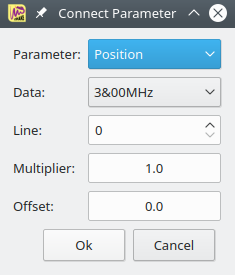
\includegraphics[width=0.3\linewidth]{Images/ConnectPars.png}
\end{center}

Here several values need to put in:
\begin{itemize}
  \item Parameter: the name of the parameter that should be linked to
  \item Data: the name of the fitting data tab that should be linked to
  \item Line: the number of the row that should be linked to (first row is `0')
  \item Multiplier: multiply the linked value by this number
  \item Offset: offset the linked value by this number
\end{itemize}
When doing this, the original parameter is replaced with the number `$\text{Multiplier} \cdot x +
\text{Offset}$' during the fit (with $x$ the value of the parameter that is linked to).

When pushing `Ok' in the pop-up window, the original value in the input box is replaced by a value
like `('Integral', 0, 1.0, 0.0, 0)'. The input represents: ('Par name', Line, Multiplier, Offset,
Data index) The pop-up menu is essentially an easy tool to create this input.

Note that chain-linking parameters will lead to errors. That is, do not link \texttt{par2} to
\texttt{par1}, and \texttt{par3}
to \texttt{par2}. Always refer to the original parameter (link \texttt{par2} to \texttt{par1}, and
\texttt{par3} to \texttt{par1}).

A tutorial on fitting using connected parameters can be found in the `MultiFitQuadrupole' advanced
tutorial. 


\subsection{Simultaneous fitting of multiple data sources}
Apart from connecting parameters during a fit, as described in the previous section, ssNake also
allows for the simultaneous fit of multiple data sources (i.e. spectra or time series). When fitting
in such a case, ssNake tries to minimize the difference between all the experimental and simulated
data. Fitting multiple data simultaneously only makes sense if there are connected parameters between
the fitting parameters of the different data sets (otherwise the results are identical to the case
where each data set is fit individually).

When in a fitting window, extra data can be added using the `+Add data+' tab that can be found in
the vertical tabs on the left hand side of the window. Clicking this prompts a pop-up window, where
the workspace name and the desired fitting routine can must be supplied. The new data tab will be
added to the vertical tab bar.

The new data will have its own parameters. Note that in the `extra' fitting tabs, several buttons are
missing. These are universal buttons, which are only displayed in the first (i.e. master) fitting
tab. Pushing `Fit' fits all the data sets simultaneously.

Be very careful with the vertical scaling of the spectra. If spectrum1 has 10000x more intensity
than spectrum2, spectrum2 will be almost ignored during the fit. To avoid this, scale the spectra to
have the same integral (scaling can be done via Matrix $\longrightarrow$ Normalize), or to have the
same noise intensity. Tread carefully\ldots

A tutorial on simultaneous fitting of multiple data sets can be found in the `MultiFitQuadrupole' advanced
tutorial. 

\subsection{S/N}
S/N (or SNR) calculates the signal-to-noise ratio between a defined section of noise, and a peak. SNR is a useful way to describe the quality of a spectrum, with too low values being a sign for inaccurate data. In ssNake, opening the S/N tool creates a window, in which the limits of the section of noise has to be set, as well as the region with the peak of interest. Left clicking in the plot can set these values (noise limits first, then signal limits). Note that it is essential that the region that is specified as `noise' really is noise. Any remaining signal will disrupt the SNR calculation. When the limits are set, ssNake directly calculates the SNR, using:
\begin{equation}
\text{SNR} = a_\text{max} / \text{std(NoiseRange)}
\end{equation}
with $a_\text{max}$ the maximum value within the range with the signal, and $\text{std(NoiseRange)}$ the standard deviation of the noise.

\subsection{FWHM}
FWHM, or Full Width at Half Maximum, is a tool to calculated the width of a peak. Selecting the tool in the menu creates a window, in which the boundaries of the peak of interest have to be set, for ssNake to search for the width of the peak. Make sure that there is only one peak in the selected window, otherwise the result might be inaccurate. The easiest way to select the regions is by left clicking in the spectrum. After valid input is given, ssNake directly calculates the FWHM in the units of the current axis. The order of input of the two limits is not important for the eventual calculation.

\subsection{Centre of Mass}
Calculates the centre of mass of a selected part of a spectrum or FID. For a symmetric peak, this is equal to the centre of the peak. However, for an asymmetric peak, identifying the centre is not possible via visual methods and a centre of mass calculation is required. Opening the tool creates an input window, in which the limits have to be set (as with the FWHM tool). After these are set, the centre of mass is calculated in units of the current axis, using:
\begin{equation}
R = \frac{1}{M} \sum_i y_i \cdot x_i  \quad,
\end{equation}
with $M = \sum y_i$ and $y_i$ the y-value corresponding to x-value $x_i$.

\subsection{Integrals}
Using this tool, integral values of selected regions of the spectrum can be obtained. Click on the
left and right side of a peak integrates this region, and displays the integral in the window, as
well as drawing a curve in the plot. By overwriting one of the obtained integral values, all the
results can be scaled: setting the first integral to 1 shows all the integrals relative to the first
integral.

\subsection{Relaxation Curve}
This routine can be used to fit relaxation curves of time-domain data (T$_1$,T$_2$). The equation
used for this is:
\begin{equation}
  y = \text{amp} \cdot (\text{const} + \text{coeff} \cdot \exp(-x/\text{T}))
\end{equation}
The standard values in ssNake are $\text{const} = 1$ and $\text{coeff} = -1$, which are generally
used in case of a saturation recovery T$_1$ measurement. For inversion recovery,  $\text{const} = 1$
and $\text{coeff} = -2$. In case of a T$_2$ experiment:  $\text{const} = 0$
and $\text{coeff} = 1$.

The axes of the plot can be set to a logarithmic scale. Negative number will not be shown in this
view. When switching to the log axis, sometimes a recalculation of the curve is necessary to get a
nice plot.


\subsection{Diffusion Curve}
This routine can be used to fit diffusion curves. The equation
used for this is:
\begin{equation}
   y = \text{amp} \cdot (\text{const} + \text{coeff} \cdot \exp(-(2\pi\gamma  \delta  x)^2  D  (\Delta -\delta / 3.0)))
\end{equation}
Here, $\gamma$ represent the $\gamma$-value of the isotope that is measured in Hz/T, $\delta$ is the length
of the gradient pulse, $\Delta$ is the time between the gradient pulses (i.e. the time from the
start of gradient pulse 1, to the start of gradient pulse 2). $D$ is the diffusion constant, which
is what we will fit. The `const' and `coeff' parameters have the same meaning as in the relaxation
curve fit. Note that the $x$-axis should be in terms of the gradient strength (in Tesla/metre). ssNake
will still show `seconds' as a unit though (1 s = 1 T/m).




\subsection{CSA}
This fitting routine can be used to simulate lineshapes influence by chemical shift anisotropy
(CSA), in both the static case, and under both infinite and finite MAS. An iterative fitting
procedure is used for the fitting, so the initial guess should be somewhat close to the optimal
solution. General values that need to be set are:
\begin{itemize}
\item The Cheng number (number of powder averages)
\item The definition: the used chemical shift definition (see the part on on the CSA Utility for more information)
\item The background (constant value added to all data points)
\item The MAS method: static, finite or infinite
\item The spinning speed in kHz (when MAS is on `finite').
\item The number of sidebands (when MAS is on `finite'). This value must always be larger then the
  expected number of spinning sidebands. When too few sidebands are simulated, the sideband intensities will be off. 
Larger values take more time to simulate. For efficiency powers of two should be used.
\item The rotor angle in radian (when MAS is not static). Default is the magic angle:
	 $\text{arctan}(\sqrt{2})$
\end{itemize}
And for each site:
\begin{itemize}
\item The three chemical shift values (depend on the definition) in units of the current axis.
\item Integral: total integral of the lineshape
\item Lorentz: amount of Lorentzian linebroading in Hz
\item Gauss: amount of Gaussian linebroading in units of the current axis. Note that Gauss in ppm should be used to 
            describe chemical shift distribution.
\end{itemize}
A maximum of 10 sites can be fitted simultaneously.

Peak picking can be used by left clicking on the spectrum. It takes three clicks (on different the
discontinuities) to set the three chemical shift values. Note that this can only be used in the 11-22-33 or
xx-yy-zz definition.


\subsubsection*{Equations}
The chemical shift interaction is described using the spherical tensor definitions discussed
above. The equations are simplified by assuming that the magnetic field is along $z$, and by
truncating the Hamiltonian to only parts that commute with the Zeeman interaction (i.e. commute
with $I_z$). (These are the regular approximations used in NMR)

The chemical shift has only a rank 0 and rank 2 tensor part. The terms are:

\begin{equation}
  T_{0} = \left( - \sqrt{\frac{1}{3}} I_z B_0 \right)
  \quad\quad\quad
\Lambda_0 = \left( - \gamma \sqrt{\frac{1}{3}} (\sigma_{zz} + \sigma_{xx} + \sigma_{yy}) \right)
\end{equation}
\begin{equation}
  T_{2} = \left( \begin{array}{c}
0 \\
0 \\
\sqrt{\dfrac{1}{6}} 2I_z B_0 \\
0 \\
0\\
  \end{array} \right)
  \quad\quad\quad
\Lambda_2 = \left( \begin{array}{c}
  \dfrac{1}{2} \gamma (\sigma_{xx} - \sigma_{yy})\\
  0\\
  \gamma \sqrt{\dfrac{1}{6}} (2\sigma_{zz} - \sigma_{xx} - \sigma_{yy})\\
  0\\
  \dfrac{1}{2} \gamma (\sigma_{xx} - \sigma_{yy})\\
  \end{array} \right)
\end{equation}

Here, it is clear that the rank 0 term accounts for the isotropic chemical shift, while the rank 2
terms hold the anisotropic information. To calculate the actually NMR frequencies, the difference
between the $I_z$ value of two energy levels should be used. This is usually 1, as only single
quantum transitions are observed.



\subsection{Quadrupole}
This fitting routine can be used to fit powder lineshapes of quadrupoles of any spin quantum number,
either static, or under spinning (with finite or infinite spinning speed). Satellite transitions can
be turned on or of. General values that need to be set are:
\begin{itemize}
\item The spin quantum number $I$ 
\item The MAS type: static, finite MAS or infinite MAS
\item The satellites (on or off, note that for integer $I$ values, they must be on)
\item The Cheng number (number of powder averages)
\item The rotor angle in radian (when MAS is not `static'). Default is the magic angle:
	 $\text{arctan}(\sqrt{2})$
\item The number of sidebands (when MAS is on `finite'). This value must always be larger then the
  expected number of spinning sidebands. When too few sidebands are simulated, the sideband intensities 
will be off. Larger values take more time to simulate. For efficiency powers of two should be used.
\item The spinning speed in kHz (when MAS is on `finite').
\item The background (constant value added to all data points)
\end{itemize}
And for each site:
\begin{itemize}
\item Position: centre of the lineshape in units of the current axis. This value is added to all 
          $x$-values from the simulation. 
\item $C_\text{Q}$: quadrupolar coupling constant in MHz.
\item $\eta$: the asymmetry parameter
\item Integral: total integral of the lineshape
\item Lorentz: amount of Lorentzian linebroading of the central transition in Hz
\item LorentzST: amount of Lorentzian linebroading of satellite transitions in Hz
\item Gauss: amount of Gaussian linebroading in units of the current axis. In ppm unit Gauss can 
describe chemical shift distribution
\end{itemize}
A maximum of 10 sites can be fitted simultaneously.

When simulating an infinite MAS spectrum, a more efficient routine can be used than for finite MAS.
If spinning sidebands are not important in the calculation, it might be useful to switch to
`infinite' for speed considerations.







\subsubsection*{Equations}
Quadrupole systems are influenced by both the first and second order quadrupolar coupling. The first
order quadrupolar coupling has only rank 2 terms, while the second order has rank 0, 2 and 4
terms.

\textit{First order:}
\begin{equation}
  T_{2} = \left( \begin{array}{c}
0 \\
0 \\
3 I_z^2 - I (I+1) \\
0 \\
0\\
  \end{array} \right)
  \quad\quad\quad
  \Lambda_2 = \dfrac{C_\text{Q}}{4  I (2 I - 1)} \left( \begin{array}{c}
  \sqrt{\dfrac{1}{6}} \eta\\
  0\\
  1\\
  0\\
  \sqrt{\dfrac{1}{6}} \eta\\
  \end{array} \right)
\end{equation}


\textit{Second order:}
\begin{equation}
  T_{0} = \left( I_z (I(I+1)-3 I_z^2) \right)
  \quad\quad\quad
  \Lambda_{0} = B \left( -\dfrac{1}{5} (3 + \eta^2) \right)
\end{equation}

\begin{equation}
  T_{2} = \left( \begin{array}{c}
0 \\
0 \\
I_z (8 I (I + 1) -12 I_z^2 - 3) \\
0 \\
0\\
  \end{array} \right)
  \quad\quad\quad
  \Lambda_{2} = B \left( \begin{array}{c}
\dfrac{1}{7} \sqrt{\dfrac{3}{2}} \eta \\
0 \\
\dfrac{1}{14} (\eta^2 - 3) \\
0 \\
\dfrac{1}{7} \sqrt{\dfrac{3}{2}} \eta\\
  \end{array} \right)
\end{equation}

\begin{equation}
  T_{4} = \left( \begin{array}{c}
0 \\
0 \\
0 \\
0 \\
I_z (18 I (I + 1) -34 I_z^2 -5) \\
0 \\
0\\
0 \\
0 \\
  \end{array} \right)
  \quad\quad\quad
  \Lambda_{4} = B
  \left( \begin{array}{c}
\dfrac{1}{4 \sqrt{70}} \eta^2 \\
0 \\
\dfrac{3}{70}  \sqrt{\dfrac{5}{2}} \eta\\
0 \\
 \dfrac{1}{140} (18  + \eta^2) \\
0 \\
\dfrac{3}{70}  \sqrt{\dfrac{5}{2}} \eta\\
0 \\
\dfrac{1}{4 \sqrt{70}} \eta^2 \\
  \end{array} \right)
\end{equation}


With $B = \left( \dfrac{C_\text{Q}}{4 I (2 I - 1)} \right) ^ 2  \dfrac{2}{\nu_0}$, where $\nu_0$ is
the Larmor frequency of the nucleus.


\subsection{Quadrupole+CSA}
Quadrupole + CSA fitting combines first and second order quadrupolar effects and chemical shift anisotropy. 
Both spinning and static spectra can be simulated. For the effects of the individual quadrupole or CSA 
settings, see above at their respective sections.

Three additional parameters that need to be given are the three angles defining the rotation of the CSA 
tensor with respect to the EFG tensor ($\alpha$, $\beta$, $\gamma$).
We order the EFG tensor values in the following way: $|V_{zz}|>|V_{xx}|>|V_{yy}|$.
We define the CSA and quadrupole angles in the same way as SIMPSON does, but we rotate via
an Z-X-Z euler rotation, while SIMPSON uses Z-Y-Z. This leads to the following conversion table, showing 
the ssNake angles when using $\alpha$, $\beta$, $\gamma$ in another software package:

\begin{center}
\begin{tabular}{cc}
\toprule
\textbf{Software} & \textbf{ssNake equivalent}\\
\midrule
Simpson & $\alpha + 90^\circ$, $\beta$, $\gamma + 90^\circ$ \\
wsolids & $\alpha + 90^\circ$, $\beta$, $\gamma$ \\
\bottomrule
\end{tabular}
\end{center}


\subsection{Czjzek}
This fitting routine can be used to simulate the 1D spectrum of a quadrupolar nucleus that
experiences a Czjzek distribution (normal or extended Czjzek). This fitting routine behaves
differently than the ones described above, as it uses a library for simulating the spectra. Czjzek
distributions are the sum of multiple quadrupolar spectra, with a different $C_\text{Q}$ and $\eta$
values, and scaled with the intensify that comes out of the distribution. To be able to simulate
this in a reasonable time, it is convenient to precalculate all the individual spectra (for each
$C_\text{Q}$ and $\eta$ pair). Fitting the spectrum leads to a new intensity distribution for each
iteration, which, using the spectrum library, can easily be used to construct the Czjzek spectrum.

Using this fitting routine, first requires the generation of a library. Using the `Library'
button, a window is opened, in which some general quadrupolar settings have to be set (see the part
about regular quadrupolar fitting). Apart from that, the $C_\text{Q}$ and $\eta$ grid have to be
set: number of steps and minimum/maximum for each parameter. Note that the values of these parameters
depend on the Czjzek distribution that is to be calculated (i.e. the $\sigma$ value). When a
distribution with a higher $\sigma$ value is used, the largest $C_\text{Q}$ value of the distribution
should be higher, the properly sample the whole intensity distribution. To aid with this, the
current distribution of each site can be viewed in this window (press `Show' on the righthand side
of the window to draw the contour plot). Press `Generate' to generate the library, and then close
the window.

The created library can now be used to simulate Czjzek spectra. For this, the following values need
to be set:

\begin{itemize}
\item d: the order parameter (integer from 1 to 5)
\item $\sigma$: the width of the distribution in MHz
\end{itemize}
In case of an extended Czjzek (i.e. a distribution on top of a non-zero $C_\text{Q}$ and $\eta$
value):
\begin{itemize}
  \item $C_\text{Q}0$: the undistorted $C_\text{Q}$-value
  \item $\eta0$: the undistorted $\eta$-value
\end{itemize}
Note that the extended Czjzek values will be activated when the `Type' dropdown menu is changed to
`Extended'. Extended Czjzek distributions take a long time to simulate. 

Note that, if the parameters change much during a fit, the $C_\text{Q}$ and $\eta$ range of the
Library might not be appropriate anymore. If this is the case, we advice to generate a new library
with better settings, and then rerun the fit, to get the final convergence.


\subsubsection*{Equations}

The normal Czjzek distribution is defined as \cite{Grimminck2011Easy}:
\begin{equation}
  A(C_\text{Q},\eta) = \frac{C_\text{Q}{}^{d - 1} \cdot \eta}{\sqrt{2\pi} \cdot \sigma^d} (1 - \eta^2 / 9) \cdot
  \exp\left[\frac{-C_\text{Q}^2 (1 + \eta^2/3)} {2\sigma^2}   \right]
\end{equation}
This equation gives the amplitude $A$ for a specific $C_\text{Q}$, $\eta$, $\sigma$ and $d$. ssNake
scales the amplitude distribution to make the sum equal to 1.


For the extended Czjzek:
\begin{align}
  A(C_\text{Q},\eta) = & \frac{C_\text{Q}{}^{d-1}}{\sigma^d} \eta \left(1 - \frac{\eta^2}{9} \right)
  \int \int \int \sin(\beta) \text{d}\alpha \text{d}\beta \text{d}\gamma \nonumber \\
  & \exp \left\{ -\frac{1}{2\sigma^2} \left[ C_\text{Q,0}^2 \left(1 + \frac{\eta_0^2}{3}\right) +
  C_\text{Q}^2 \left(1+ \frac{\eta^2}{3}\right) \right.\right. \\
  & \left.\vphantom{\frac{a^1}{1}} \left.\vphantom{\frac{a^1}{1}} - \frac{2}{\sqrt{3}} C_\text{Q} C_\text{Q,0} 
  \left( \sqrt{3} a_{11} + \eta_0 a_{15} + \eta \left(
 a_{51} + \frac{\eta_0 a_{55}}{\sqrt{3}} \right) \right) \right] \right\} \nonumber
\end{align}
with
\begin{align}
  a_{11} = & \frac{1}{2} (3\cos^2\beta - 1)\\
  a_{15} = & \frac{\sqrt{3}}{2} \sin^2\beta \cos 2\alpha \\
  a_{51} = & \frac{\sqrt{3}}{2} \sin^2\beta \cos 2\gamma \\
  a_{55} = & \frac{1}{2} \cos 2\alpha (1 + \cos^2\beta) \cos2\gamma - \sin 2 \alpha \cos \beta \sin
  2 \gamma.
\end{align}
In this case, integration over three angles is required, which makes the calculation quite involved
(and therefore slow). For the special case $\eta_0=0$, a faster equation can be used:

\begin{align}
  A(C_\text{Q},\eta) = & \frac{C_\text{Q}{}^{d-1}}{\sigma^d} \eta \left(1 - \frac{\eta^2}{9} \right)
  \exp \left\{ - \frac{C_\text{Q,0}^2 + C_\text{Q}^2 (1 + \frac{\eta^2}{3})}{2\sigma^2} \right\}\\
  & \cdot \int_0^1 I_0(z) \exp \left\{ \frac{C_\text{Q}C_\text{Q,0}}{2\sigma^2} (3t^2 - 1)   \right\} \text{d}t
\end{align}
with $I_0(z)$ a modified Bessel function, and
\begin{equation}
  z = \eta \left| \frac{C_\text{Q}C_\text{Q,0}}{2\sigma^2}\right| (1 - t^2)
\end{equation}

To speed-up the calculations of these distributions, ssNake can use the \texttt{numba} python library. With
the extended Czjzek distribution, around a twofold speed increase can be gained in this way. ssNake
tests for the \texttt{numba} package itself, so regular installation of this package should be sufficient.

\subsection{MQMAS}
This fitting routine can be used to fit an MQMAS spectrum. It is a 2D fitting routine, showing a contour plot 
of the data. The fit result is plot on top of this using a different contour colour. Related to the additional dimension
a Lorentz1 parameter is added to describe relaxation in D1. Regardin Gaussian broadening, Gauss parameter is used in 
both dimensions to describe chemical shift distribution.

For simulation of MQMAS data, we need to define the quadrupolar parameters as before (see the section on fitting 
of quadrupole lines). In this case, no satellite signals are included. Only infinite MAS spinning speeds are
 supported (no spinning sidebands are calculated). Moreover, it is an ideal simulation, so no excitation profiles 
are taken into account.

Apart from the spin quantum number I, MQMAS simulation also requires selected the multiple quantum transition 
evolving in D1 to be supplied. This is labelled `MQ' in the interface. 

Two additional parameters that need to be supplied are the shearing and spectral width scale factors. These allow 
to model 2D MQMAS spectra processed using diferent shearing schemes. Check our advanced tutorial on MQMAS processing. 
By default, the shearing is set at 0, and the sw scaling at 1. This results in unsheared data with D1 corresponding 
to 3Q coherence evolution, and can be used to fit experimental data that has not been sheared.

The required sharing and sw scaling factors depend on both I and MQ. Using the 'Auto' push button in the interface, 
the correct values are filled in in the boxes, depending on the current I and MQ setting.


\subsection{Czjzek MQMAS}
This routine can be used to fit an MQMAS spectrum of a species that is influenced by a Czjzek distribution. The 
required inputs are describe in the section on 1D Czjzek fitting, and regular MQMAS fitting respectively. Note 
that this again means that firstly a library needs to be generated of a $C_\text{Q}$ and $\eta$ grid. The spectrum 
sharing and sw scaling are as described in the MQMAS section.


\subsection{External}
Simulating NMR data for fitting can be straightforward, if idealized line shapes are requires. These
type of calculation are programmed into ssNake, and can be run using the different tools described
above. However, if actual pulse sequences need to be calculated, the simulations become involved
quite quickly. In order ot be able to fit spectra wich require a more involved calculation, the
`External' tool can be used to fit spectra using external programs.


Here we provide an example on how to use this tool together with the SIMPSON package\cite{Bak2000SIMPSON,Tosner2014Computer,Tosner2009Optimal}.
For this, a SIMPSON input script is
required which gives a single spectrum/FID as output. ssNake then loads this data, applies a Fourier
transfrom (if necessary) and regrids the data to have the same $x$-axis as the experimental data.

As with the `Function Fit' described below, the variables that we want to fit (or change) in the
ssNake fit window must be defined as `@a@' in the SIMPSON input file (were $a$ can be any name). ssNake
then recognizes the different variables defined in this way. When a simulation is run, ssNake
replaces these variable names by the relevant number and performs a SIMPSON simulation using this
input script. By default, ssNake also adds a scale factor, and Lorentzian and Gaussian apodization
input boxes.

The window also features a dropdown box for the number of sites. When increasing this, new input
boxes for all the relevant primate's appear. Note that ssNake is now running SIMPSON multiple times
for each simulation: once for each site. Note that it is also possible to make SIMPSON run
simulations with multiple sites in one go, but that this is really inefficient. Naturally, when
spin-spin interactions are present (dipolar, J) the relevant spins \textit{should} be included in a single
SIMPSON file.


If, for example, we want to fit the chemical shift anisotropy ($\delta_\text{aniso}$) and asymmetry ($\eta$), 
($\delta_\text{aniso}$) and asymmetry ($\eta$), we could use the following SIMPSON spinsys:

\lstset{language=tcl}          % Set your language (you can change the language for each code-block optionally)

\begin{lstlisting}[frame=single]  % Start your code-block

spinsys {
    channels	1H
    nuclei	1H
    shift	1 100 @aniso@ @eta@ 0 0 0
}
\end{lstlisting}
Here, the isotropic shift ($\delta_\text{iso}$) has been fixed at 100 Hz, while the anisotropy and
eta can be changed from within ssNake. Note that the @$a$@ variables can be used anywhere in the
input file. Also, the used names can be anything (but be careful with special characters), but names
like `a' or `agdv' might be difficult to recognise for the user in the ssNake window.
A full input file could look like:

\begin{lstlisting}[frame=single]  % Start your code-block

spinsys {
    channels	1H
    nuclei	1H
    shift	1 100 @aniso@ @eta@ 0 0 0
}

par {
	proton_frequency	600e6
	method 			direct
	sw			1E6
	variable np		512
	crystal_file	  	zcw232
	gamma_angles		1
	start_operator		Inx
	detect_operator		Inp
	verbose			0000
	spin_rate 		0
}

proc pulseq {} {
   global par
   delay [expr 1e6/$par(sw)]
   store 1
   reset
   acq $par(np) 1 0
}

proc main {} {
   global par
   set f [fsimpson]
   fzerofill $f 16384
   fft $f
   fsave $f $par(name).spe
}
\end{lstlisting}
Note that, when external files like user crystal files are used, the full path to this file must be
included in the input file (ssNake copies the input file to a random directory, without any
required files).

SIMPSON calulations can take a very long time. We therefore suggest to always optimze the input file
as much as possible (minimum number of points and crystal orientations).




\subsection{Function fit}
While we try and include as  many relevant fit function as possible, we cannot include everything in
ssNake. In cases were the supplied functions are not useful, `Function fit' can be used. Using this
window, a function input by the user can be supplied. Pushing the `Input Function' button opens a
window were the required function can be supplied. The $x$-variable is the $x$-axis, and other
variable can be supplied by the @$a$@ notation (with $a$ any variable name you like, with no special
characters in the name). For example, let us say we want to fit a parabola with an offset. This would look like:
\begin{equation}
  x ** 2 * @a@ + @b@
\end{equation}
with $a$ and $b$ the variable to be fit. Note the Python way of writing the square of $x$ is $x **
2$. Pushing Ok will load the function, and display $a$ and $b$ for the user to input (or fit). Note
that the `@' signs are only used by ssNake to recognise which are variable in the equation.


\section{Combine}
The combine menu options allow the interaction between different workspaces like multiplication and addition. For some of these tools it is essential that the workspaces
are the same size, or can be broadcasted. Broadcasting is described below.

\subsection{Broadcasting}
ssNake makes use of the general broadcasting rules of the numpy python package. Generally, data that has less dimensions than the target can be added (multiplied, etc)
if the last dimensions agree on size. For example, 3x1024 can be added to 2x3x1024 (the data is just stretched along a new third dimension). Alternatively, data that has a size 1
along a specific dimension can also be added: 2x1x1024 added to 2x10x1024 (again, the data is copied in the second dimension to reach length 10).
Note that always the last dimensions are checked, so adding 1024x3 to 1024x3x10 is not possible: checking is done from the right.

\subsection{Combine Workspaces}
Using Combine Workspaces opens a window that allows for the selection of multiple workspaces via dragging and dropping in the right-hand list.
Only workspaces with the same size can be combined (and error will be given otherwise). The selected workspaces will be combined and copied to a new workspaces, of which the name will be asked.
Combining multiple sets of data this way requires the creation of a new dimension, which is always the new dimension D1. For example, combining two 1D data sets with 1024 points will
lead to a combined data set of 2x1024 points (D1xD2). Combining two sets of 10x512 data points leads to a 3D set of 2x10x512.


\subsection{Insert From Workspace}
Insert From Workspace can be used to append data from another workspace to the current. For this, it is \textit{not} necessary to have two Workspaces of exactly the same size.
However, appending must be possible in some way. The way the data is appended depends on the active dimension. For example: the current data has size 2x1000 and D2 is viewed.
Inserting a 1D data set of 500 points leads to a 2x1500 data set. Doing the same when viewing the D1 dimension gives an error. It would be possible to append a 1D set of 1000
points to this data from D1. This gives back a 3x1000 data set.


\subsection{Add}
Add the data of the selected workspace to the active workspace. The active dimension is not considered. Data of both workspaces must be the same size, or must be able to be broadcasted (see above).


\subsection{Subtract}
Same as add, but now subtracting.

\subsection{Multiply}
Same as add, but now multiplying the data sets. Note that ssNake by default has complex data. Using Multiply therefore does a complex multiplication.
If this is not desirable, first use Tools $\rightarrow$ Real to get rid of the imaginary part of the data.

\subsection{Divide}
Same as add, but now dividing. Note that the data is complex, as described for Multiply.




\section{Plot}
The plot menu allows the user the change the view and nature of the current data. Several types, for both 1D and 2D views are supported. Apart from the view, the current x-axis can be changed, and a
frequency reference can be set and saved.


\subsection{1D Plot}
Shows the default 1D plot with a solid line. The side window only shows the dimension selector, as there are no additional options.


\subsection{Scatter Plot}
This plot type is essentially the same as the 1D Plot. However, the data is now plot as points without a line. Scatter plots can be useful for viewing
plots with only a couple of points.

\subsection{Stack Plot}
A stack plot is a way to view 2D data. Every trace is plot as a separate line, with a certain y-offset depending on its number. The y-axis in this view must be view with care,
due to the offset given to each trace. In a stack plot, the dimension selector show two bullets: a left one for the main view, and the right one for the stack. For a T1 array, for example, having D2 as the first, and D1
as the right bullet shows a plot of the data along D2, with a separate spectrum (or FID) for every point in D1 (the arrayed recovery time in this case).

The side frame shows several options:
\begin{itemize}
  \item From: index from where to start with the stack (zero is the start).
  \item To: index where to stop with the stack. Note that this should be 1 higher than the last point (it is to not including the shown value)
  \item Step: step size of the From to To array. 1 shows every spectrum, 2 only every second spectrum, etc.
  \item Spacing: the distance in units of y between each spectrum (or FID). This can also be scrolled using <shift -- scroll>.
\end{itemize}

\subsection{Array Plot}
This plot is essentially the same as the Stack Plot, only now the spectra are plot next to each other. In this case, the labels of the x-axis are
not shown anymore, as the do not make any sense. The label of the x-axis is changed to `Frequency' or `Time' to indicate a series of spectra or FID's.
The x-limits of every subplot are taken from the view before changing to the Array Plot, and cannot be changed from the array plot.

The settings in the side frame are the same as with the Stack Plot.


\subsection{Contour Plot}
A contour plot shows the height profile of the data using constant height lines (like altitude lines on a
map). This is the most common way to view true 2D data (data in which there are two NMR dimension, which are
both Fourier transformed). Calculation of the contour lines takes some time, especially for larger data sets.
As with the Stack and Array plot, the dimension selector shows two bullets. Now they stand for the x-axis
(left) and y-axis (right). The Get Position frame now shows some extra features, as each data point now has a
x-value, y-value and amplitude (z-value). Note that you can change the colour scheme of the contour plot under
Plot $\rightarrow$ Plot Settings.

The side frame has several options, which are described below.

\subsubsection*{Contour type}
\begin{itemize}
  \item \textit{Number}: the number of contour lines plot. Positive and negative lines are treated separately (so the real maximum is twice this number). Also, when
	 the multiplier type is chosen, the total number of lines depends on whether or not the level maximum is exceeded.
  \item \textit{Sign}: whether or not to plot only the positive contours (+ only), only the negative ($-$ only) or both (Both).
  \item \textit{Type}: Linear or multiplier. Linear has even spacing between the contour lines, and goes in `Number' steps from the contour minimum to the
	 maximum (for both the negative and positive contours). Multiplier takes the lowest contour and multiplies it with the Multiplier to get the 2nd contour. This is continues
	 until the contour maximum, or the maximum number of lines is reached.
  \item \textit{Multiplier (optional)}: Supplies the multiplier value as described above.
\end{itemize}


\subsubsection*{Contour limits [\%]}
Sets the maximum and minimum contour. The maximum cannot be higher than 100\%, and the minimum
cannot be lower than 0\%. Whenever the minimum is higher than the maximum, the meaning (but not the
labels) is interchanged. The minimum contour level can be scrolled using the <shift -- scroll> with
the mouse wheel.

Two types are supported via the `Rel.\ to.' dropdown menu: `Current 2D' and `Full data'. `Current
2D' sets the 100 \% value of the contours equal to the maximum of the current shown 2D plot. `Full
data' displays it relative to the maximum of the entire dataset. This last option is particularly
handy when view 3D data, were traces with no intensity compared to the data maximum are irrelevant,
and should not show any contour levels.

\subsubsection*{Projections}
The projections are the regular 1D plots shown at the top and right of the contour plot. These can be of help in viewing the data.
For both, several types are available:
\begin{itemize}
  \item Sum: the sum of the data
  \item Max: the maximum of the data
  \item Min: the minimum of the data
  \item Off: no projection is displayed
  \item Trace: value of a particular trace
\end{itemize}
Sum, Max, and Min are applied along the axis opposite to the projection. So the top projection
(which shows the x-axis) is summed (max/min) along the y-axis.

Alternatively, the Projection Ranges box can be toggled. This allows the user to specify between
which data points the operation (sum/min/max) should be applied.  This can be useful to get higher
signal-to-noise level projections, by preventing contributions from noise-only areas.

The `Trace' option sets the projection equal to a particular line in the 2D data. Using the `Select
Traces' button, a trace can be selected by clicking in the contour plot.

\subsubsection*{Diagonal}
Ticking this box draws a diagonal line across the 2D data at x = y. Note that the axis type is of importance: no scaling is performed.
Therefore, if a data set with two identical axes is plot, only if the two units are the same, the diagonal is plot in a way that (probably) is the correct way.
Alternatively, there is a box called `Multiplier', in which a value can be put that multiplies the x-axis (only for the calculation of the diagonal).

\subsection{Multi Contour Plot}
This plot type can be used to plot several contour plots in the same image. It works in a similar way as the Multi plot described below. In this case, a shift in both the x and the y-axis can be supplied.

Each data set is plot using a constant contour colour, with a lighter colour representing negative contours.

\subsection{2D Colour Plot}
A 2D Colour plot shows the height profile of the data using a colour scheme.
This plot type essentially show the same information as a Contour plot, but might
be more applicable for certain types of data. It is used often for viewing NMR imaging (MRI) data.

As with the Contour plot, the 2D Colour plot shows projections, of which the settings can be changed in the side frame (see the Section on Contour Plot for more information).

The colour scheme of the plot can be changed in the plot settings, or in the general preferences.

\subsection{Multi plot}
A multi plot is on overlay of multiple workspaces. It shows the 1D Plot of the active workspace, and a button
to add additional data (from other, or the same workspace). Things that can be changed are:
\begin{itemize}
  \item Scale: linear multiplier of the signal ($y$ value)
  \item Offset: gives a vertical offset to the current data. The step size depends on the data, and is shown between
	 brackets.
  \item Shift: horizontal shift in units of the current axis.
  \item Dimension selector: selects the dimension and trace to be shown (as with a regular 1D plot).
\end{itemize}
The added data can be removed by pushing the `x' button.


\subsection{User X-axis}
This function opens a window were the current axis can be changed. This is commonly done in the time domain
for relaxation data (as the axis is probably non-linear). The possible inputs are described below. Pushing OK
applies the axis to the current data. To preview it, push enter while in on of the input boxes. The values are
then printed in the table below.

Note that several actions on the data reset the $x$-axis (Fourier transform, for example). This is because
these processes can only use the default axis. It is therefore wise to set the $x$-axis after all processing is
done (i.e. before fitting, or printing a figure).

\subsubsection{Expression}
Allows input of a list of values via an input box. Allowed inputs are any \texttt{Python} commands that lead
to a list of the correct length. Alternatively a space separated input can be given, e.g.: 0 0.1 0.2 0.4.

One extra command that we have included and regularly use is the `euro' command. For relaxation measurements a
list that follows the series of the euro coins is easy to remember and convenient. The series always start at
1, 2 or 5 (or 10 times lower/higher values). Having a euro series of length 5 starting at 0.1 therefore gives:
0.1, 0.2, 0.5, 1, 2. The euro series can be created with the command `euro($y$)' with $y$ the start value of
the series.



\subsubsection{Linear}
A regular linear spacing. The start and end value needs to be supplied.

\subsubsection{Logarithmic}
A logarithmic spacing. The start and end value need to be supplied (and ssNake calculates the spacing). Not
that negative values are not allowed.

\subsection{Plot Settings}
This open a window were the plot settings of the active workspace can be changed. The input value are explained
at File $\rightarrow$ Preferences.


\section{History}
\subsection{History}
Whenever ssNake performs an action on the data, a line is added to the history list to be able to show the processing history. In the History menu, these
entries can be viewed. Saving the data (to a JSON or MATLAB file) also saves the history (but not the undo information). Note that changing the view of the data
is not an action, nor is fitting the data. Changing the spectral width and such \textit{is} considered an action.


\subsection{Error Messages}
Whenever a wrong input is given to ssNake, a message is printed in the status bar (on the bottom of the main window). In Error Messages, these messages
can also be found (printed in black), with a time stamp of their occurrence. Apart from these warning messages, there can also be more serious issues.
These are python errors, and indicate that we did something wrong, or forgot to check if the input is correct. These messages are not displayed in the
status bar, but only in the Error Messages window. They are printed in red, and when selected show some additional information in the bottom area of this window.
Whenever a tools gives no, or an unpredictable result, consult this window for any errors. If such an error occurs you can email us with the specifics.
For this, it is useful to be able to reproduce the error, otherwise it becomes difficult to find the cause.





\section{Utilities}
\subsection{Chemical shift conversion tool}
In NMR literature there are several definitions in use for describing the chemical shift tensor. This tool provides an easy way to inter convert them. The definitions are based on the very useful website of Klaus Eichele (\url{http://anorganik.uni-tuebingen.de/klaus/nmr/index.php?p=conventions/csa/csa}). In the most useful conventions, the three tensor values $\delta_\text{xx}$, $\delta_\text{yy}$ and $\delta_\text{zz}$ are rewritten to an average value, a width and an asymmetry. Below follow the definitions of the different conventions.

The primary convention is called the `Standard Convention'. This convention just gives the three principal components of the tensor, without any restructuring, called $\delta_\text{11}$, $\delta_\text{22}$ and $\delta_\text{33}$. They are ordered in such a way that: $\delta_\text{11} \geq \delta_\text{22} \geq \delta_\text{33}$.

The second convention we call the `xyz Convention'. This is essentially the same as the Standard Convention, only the ordering is different. We now have $\delta_\text{xx}$, $\delta_\text{yy}$ and $\delta_\text{zz}$. With $|\delta_\text{zz}-\delta_\text{iso}| \geq |\delta_\text{xx}-\delta_\text{iso}| \geq |\delta_\text{yy}-\delta_\text{iso}|$. With $\delta_\text{iso}$ the isotropic value, defined as the average of the three principal components. In this definition, $\delta_\text{zz}$ is the value furthest away from the isotropic value, $\delta_\text{yy}$ the closest, and $\delta_\text{xx}$ the remaining value.

The third definition is the Haeberlen definition (or Haeberlen-Mehring-Spiess). Here, the principal components are ordered as in the xyz convention, only now they are redefined into a width, asymmetry and isotropic value. With $\delta_\text{iso} = (\delta_\text{xx} +\delta_\text{yy} +\delta_\text{zz})/3$, $\delta_\text{aniso} = \delta_\text{zz} -\delta_\text{iso}$ and $\eta = (\delta_\text{yy}-\delta_\text{xx})/\delta_\text{aniso}$. This way, the asymmetry parameter $\eta$ always lies between 0 and 1. Not that due to the ordering of the principal components, the sign of the anisotropy (i.e. the width) is ill defined for $\eta=1$.

The final definition is the Herzfeld-Berger definition. This convention uses the Standard Convention as a basis, and then defines the isotropic value as $\delta_\text{iso} = (\delta_\text{11} + \delta_\text{22} + \delta_\text{33})/3$, the span as $\Omega = \delta_\text{11} - \delta_\text{33}$ and the skew as $\kappa = 3(\delta_\text{22}-\delta_\text{iso})/\Omega$. This way, the span is always positive, while the skew lies between -1 and 1.



\subsubsection*{Use of the tool}
Using the chemical shift conversion tool is quite easy. You can fill in all the necessary values for one convention, and push the `Go' button next to it to convert it to all the other definitions. Note that ssNake also checks the definitions. So if you mess up the order of the Standard Convention, for example, it will be put in the correct order. The same is done for values that are outside the defined limits (e.g. $\eta$ and $\kappa$). Pushing `Reset' will reset all the values to 0.

\subsection{Quadrupole coupling conversion tool}
Nuclei with a spin quantum number greater than 1/2 have an asymmetric charge distribution. This leads to a quadrupolar moment, and thus to a coupling between the nucleus and the electronic field gradient at the nuclear site. Just as for chemical shift, there are multiple convention in use to describe the resulting quadrupolar tensor. Apart from being a symmetric tensor, Laplace relation states that the sum of the field gradients in all direction should be zero (otherwise the nuclei would experience a net force). Due to this, there is no isotropic term, and the quadrupolar coupling can be described by two numbers: the strength and the asymmetry. Of these there are two conventions in use: C$_\text{Q}$ and $\omegaup_\text{Q}$. When the field gradients in the three independent directions are $V_\text{xx}$, $V_\text{yy}$ and $V_\text{xx}$ (with $|V_\text{zz}| \geq |V_\text{xx}| \geq |V_\text{yy}|$), C$_\text{Q}$ is defined as:
\begin{equation}
C_\text{Q} = \dfrac{eV_\text{zz}Q}{\hbar} = \dfrac{e^2qQ}{\hbar}
\end{equation}
or the more commonly used C$_\text{Q}/2\piup$ (which has Hz as unit):
\begin{equation}
C_\text{Q}/2\piup = \dfrac{eV_\text{zz}Q}{h} = \dfrac{e^2qQ}{h} \quad .
\end{equation}
With $e$ the elementary charge, $Q$ the quadrupole moment (in m$^2$), $h$ the Planck constant (and $\hbar$ the reduced Planck constant). Alternatively, a value that is scaled with the spin quantum number $I$ is used:
\begin{equation}
\omegaup_\text{Q}/2\piup = \dfrac{3e^2qQ}{2I(2I+1)h} = \dfrac{3}{2I(2I+1)} C_\text{Q}/2\piup	\quad .
\end{equation}
For both definitions, the asymmetry is defined as:
\begin{equation}
\eta = \dfrac{V_\text{yy} -V_\text{xx}}{V_\text{zz}}
\end{equation}
which, due to the ordering of the fields gradient components, is always between 1 and 0.

Generally, only the $C_\text{Q}$ and $\omegaup_\text{Q}$ definitions are used, and the field gradients themselves are not shown. However, if the quadrupolar coupling for a nucleus in a material is known, the field gradients can be calculated by using the known quadrupolar moment of the nucleus. This way, the quadrupole coupling for another isotope at the same site in the material can be calculated by reversing the equation with a new moment and spin quantum number.

\subsubsection*{Use of the tool}
Using the quadrupole conversion tool is quite easy. You can fill in all the necessary values for one convention, and push the `Go' button next to it to convert it to all the other definitions. Note that ssNake also checks the definitions. So if you have an asymmetry below 0, it will reorder the field gradients in such a way it lies between 1 and 0 again. To calculate the field gradients from the quadrupole coupling constant (or the other way around), the quadrupolar moment should be given (which starts at `ND", being `not defined'). When starting from the field gradients, ssNake checks if they sum to 0 (which they should). If not, the difference is subtracted from the three values, to make sure it is. Note that only the absolute quadrupolar coupling is found in NMR, so pay no heed to the absolute sign of the field gradients.


\subsection{NMR table}
This tool provides an interactive way to find and calculate NMR frequencies and other characteristic
values. The main view is the periodic table, showing the NMR frequency in MHz at a specific magnetic
field for the most common isotope of each element. Changing one of the values (and pressing enter)
updates all other values. Most commonly, either the B$_0$ field (in the top left corner) or the
$^1$H frequency is supplied by the user. Each element also has a coloured box representing the spin
quantum number (of the most common isotope). Apart from the B$_0$ field, the top left corner also
shows the electron frequency in GHz.

Additional details on specific element can be obtained by double clicking on the element title, or
by clicking the `Details' button. This
creates a pop-up box showing these details. Navigating between the elements can be done from this
box via the element number or abbreviation. Show values are: \begin{itemize}
\item Mass
\item Spin quantum number (I)
\item Natural abundance and radio-active life-time (when applicable)
\item Gyromagnetic ratio ($\gamma$) in 10$^7$ rad~s$^{-1}$~T$^{-1}$
\item Quadrupole moment (Q) in fm$^2$ (when applicable)
\item NMR frequency at the given magnetic field in MHz (based on the frequency ratio $\Xi$ with
  respect to $^1$H)
\item Sensitivity relative to a specific nucleus. The sensitivity is taken to be proportional to $\gamma^3 I (I+1)$, scaled with the natural abundance.
\item Reference sample for ppm scale
\item Reference sample condition
\item Line-width factor for quadrupole nuclei ($I > 1/2$). It is defined as $\dfrac{Q^2(2I+3)}{I^2(2I-1)}$
\end{itemize}
The leftmost entry of the details window is a bullet, which can be used to set the preferred isotope
of this element in the periodic table view.

The shown frequencies are those of 0 ppm for that nucleus, at the specified magnetic field. If an
experimental frequency of TMS $^1$H is filled in the details box of $^1$H, the frequency of 0 ppm for all
other nuclei can be read from their respective boxes (in the details, where enough digits are
displayed). 






\section{Help}
\subsection{Update}
This tool can be used to update ssNake via the github page. It show a dropdown menu with all the available
versions. We recommend using that latest version (that has a version number). The `develop' version is the
version we are currency working on. This has the most resent features, but might be unstable. Note that updating via
this tool does not always work (ssNake needs write permission on its ow directory). If ssNake does not work
after using the Update tool, you can download it from the github page:
\url{https://github.com/smeerten/ssnake/}.

\subsection{About}
Opens the About box with information on the version, acknowledgements and license (GPL v3.0).

\section{Contact}
To contact the \texttt{ssNake} team write to \texttt{ssnake@science.ru.nl}.

\bibliographystyle{BibStyle}
\bibliography{ReferenceManual}

\end{document}
